%%%%% Single page layout:
\documentclass[12pt, a4paper]{article}
\usepackage[czech]{babel}
\usepackage[utf8]{inputenc}
\setlength\textwidth{145mm}
\setlength\textheight{247mm}
\setlength\oddsidemargin{15mm}
\setlength\evensidemargin{15mm}
\setlength\topmargin{0mm}
\setlength\headsep{0mm}
\setlength\headheight{0mm}
\let\openright=\clearpage

%%% Additional useful packages
% \usepackage[colorlinks]{hyperref} % reference: (Figure 1) instead of (1)  <-- \autoref{}
\usepackage{amsmath}
\usepackage{amsfonts}
\usepackage{amsthm}
\usepackage{bm}
\usepackage{graphicx}
\usepackage{psfrag}
\usepackage{fancyvrb}
\usepackage{bbding}
\usepackage{dcolumn}
\usepackage{booktabs}
\usepackage{paralist}
\usepackage{indentfirst}
\usepackage[nottoc]{tocbibind}
\usepackage{subfig} 	%subfloats.

\usepackage[font=footnotesize,labelfont={bf,sc,small},figurename=Obrázek]{caption} % change the word 'Figure' in caption
\usepackage[colorlinks=true,linkcolor=blue]{hyperref}
\renewcommand{\figureautorefname}{Obr.} % change the word 'Figure' in text
\newcommand{\subfigureautorefname}{\figureautorefname} % to make nice \autoref of the subfloats (from subfigrebui)




%%% \subref*
\captionsetup[subfigure]{subrefformat=simple,labelformat=simple,listofformat=subsimple}
\renewcommand\thesubfigure{(\alph{subfigure})}
\newcommand*{\fullref}[1]{\hyperref[{#1}]{\ref*{#1} \nameref*{#1}}} % cislo, nazev kapitoly
% \newcommand*{\fullref}[1]{\hyperref[{#1}]{\autoref*{#1} \nameref*{#1}}} % section/subsection/..., cislo, nazev kapitoly



\numberwithin{equation}{section} 	%cislovani rovnic pro article
\interfootnotelinepenalty=10000	%aby se \footnote nerozdeloval na dve strany


% ####################################################################
% ####################################################################
\begin{document}


\pagestyle{empty}
\begin{center}

\medskip

\vfill
{\bfseries\Large{Středoškolská odborná činnost}}

\medskip

{{\bfseries Obor: } 17. Filozofie, politologie a ostatní humanitní a společenskovědní obory}
\vfill


\vspace{20mm}

{\LARGE\bfseries \#filterbubble}

\vfill

\begin{tabular}{ll}
\bfseries Autoři: & Františka Sandroni\\
                  & Jakub Dostál\\
\noalign{\vspace{2mm}}
% \bfseries Konzultant: & Chceme nějakého?, UP Olomouc\\
%\bfseries Institute: & Department of Mathematical Analysis and Applications\\&  of Mathematics, Faculty of Science, Palack\'y University
\end{tabular}

\vfill
Olomouc 2017
\end{center}

% ##############################################################################
% ##############################################################################

\newpage
\openright

\noindent
\subsection*{Poděkování}
\noindent Rádi bychom poděkovali Dott. Kvidu Sandroni za projevené pozorné připomínky během celé tvorby naší práce, každá sebemenší myšlenka nám byla cennou radou a podnětem ke zdokonalování studie. Velký dík patří také Barboře Pomykalové za grafickou úpravu. Neméně děkujeme všem, kteří se ochotně podíleli na korektuře práce.


% ##############################################################################
% ##############################################################################

\newpage
% Page containing a legal statement
\vspace*{\stretch{8}}

\noindent
Prohlašujeme, že jsme tuto práci vypracovali samostatně a~výhradně
s~použitím citovaných pramenů, literatury a~dalších odborných zdrojů.

Prohlašujeme, že tištěná verze a elektronická verze soutěžní práce SOČ jsou
shodné.

\vspace{20mm}
\noindent
%% Place and date of signature
V~Olomouci dne \makebox[2.5cm]{\dotfill}
\hspace*{\fill}
\makebox[5cm]{\dotfill}
\hspace*{\fill}
\\
\\
\\
\makebox[5.55cm]{}
\hspace*{\fill}
\makebox[5cm]{\dotfill}
\hspace*{\fill}

\vspace*{\stretch{1}}

% ##############################################################################
% ##############################################################################

\newpage
%%% Czech and English abstracts
\nobreak\vbox to 0.49\vsize{
\setlength\parindent{0mm}
\setlength\parskip{5mm}
\newcommand{\forceindent}{\leavevmode{\parindent=1em\indent}}

\textbf{Title}: \#filterbubble\\
\textbf{Authors}: Františka Sandroni, Jakub Dost\'al\\
\textbf{School}: Slavonic grammar school Olomouc\\
% \textbf{Supervisor}:
% Tom\'aš F\"urst, Department of Mathematical Analysis and Applications of Mathematics, Faculty of Science, Palack\'y University Olomouc
\textbf{Abstract:}\\
Nowadays one of the mostly used source of the information are social networks. But the content user watches is adjusted by \textit{preferential algorithms}. They filter information and lead one to situation, when the content he wathes is nott fully balanced. The communities are constituted from the people with same initial opinion. This phenomena is called the \textit{filter bubble} and it causes \textbf{[[[can cause (zalezi na tom co chceme skutecne rict)]]]} creation of the extremism in the population, because it avoids users to see wide variety of opinions. And furthermore confirms the user that his opinion is the only opinion by shoving him lot of content with same orientation.\\
\forceindent We introduce the filter bubble and it's positives and negatives firstly. We present new methodology of filter bubble studying on the data from the \textit{Twitter} afterwards. The data are collected and then processed by the \textit{sentimental analysis}. In contrast to state of the art researche we are using with larger number of subjects directly from Twitter. At the end we show positive and negative features of the new methodology on few examples.\\
\textbf{[[[pokud budeme mluvit i o tom, ze trump ib nevytvari, musime pridat neco na konec abstraktu]]]}\\
\textbf{Keywords}: filterbubble, social media, sentiment analysis, democracy, society
\vss}


\vbox to 0.5\vsize{
\setlength\parindent{0mm}
\setlength\parskip{5mm}
\newcommand{\forceindent}{\leavevmode{\parindent=1em\indent}}

\textbf{Název práce}: \#filterbubble\\
\textbf{Autoři:} Františka Sandroni, Jakub Dost\'al\\
\textbf{Škola}: Slovanské gymnázium Olomouc\\
\textbf{Abstrakt:}\\
Významným zdrojem informací v dnešní době jsou sociální sítě. Obsah, který na nich jedinec pozoruje je však ovlivěn \textit{preferenčními algoritmy}. Ty filtrují informace a vedou jedince do situace, kdy okruh příspěvků, které pozoruje, není plně vyvážený. Tím pádem se zde vytvářejí komunity, jež výrazně modifikují objem a obsah informací ovlivňující jejich členy. Tomuto fenoménu se říká \textit{filter bubble} a může vést například k samovolnému vzniku extrémistických názorů a skupin, neboť jedinci v dané bublině nemají přístup k dostatečně širokému spektru informací, ale pouze k zúženému výběru.\\
\forceindent Práce nejprve představuje \textit{informační bublinu} a její positiva a negativa. Poté prezentujeme novou metodiku výzkumu informační bubliny na datech poskytovaných \textit{Twitterem}. Tato data jsou nejprve pečlivě vybrána a následně zpracována pomocí \textit{sentimentální analýzy}. Narozdíl od mnoha předešlých studií pracujeme s větším počtem subjektů a jejich konkrétním chováním na sociální síti. Funkčnost našeho modelu ukážeme na několika jednoduchých příkladech, na nichž představíme jejich kladné i záporné vlastnosti.\\
\textbf{Klíčová slova}: informační bublina, sociální sítě, sentimentální analýza, demokracie, společnost
\vss}

% ##############################################################################
% ##############################################################################

\newpage
\openright

\pagestyle{plain}
\setcounter{page}{1}

\tableofcontents

% ##############################################################################
% ##############################################################################
\newpage
\section*{Úvod}
\noindent Sociální sítě se čím dál více dostávají do popředí nejen jako volnočasové platformy pro různé aktivity, ale i~jako informační kanály. V tomto ohledu se transformují ve zdroj aktuálních zpráv z celého světa bez ohledu na to, zda jde o~novinku z uměleckých sfér, výsledky vědeckého zkoumání či seriózní informace z problematiky politických vztahů.

Aby uživatelé mohli sledovat jim imponující obsah, existují na sociálních sítích softwary umožňující filtraci uživatelem viděných příspěvků, nazývají se \textit{preferenční algoritmy}. Personalizace informačního kanálu vytváří kolem uživatele okruh pro něj obsahově zajímavých příspěvků, což v důsledku může vést do situace, kdy je obklopován stále stejnými myšlenkami a~názory. Tento fenomén byl nazván \textit{filter bubble}, neboli \textit{informační bublina} a~je doposud nepříliš prozkoumaným jevem ve společnosti. Většina studií primárně pojímá filter bubble jako fenomén na úrovni sociologie a~psychologie studující ho svými tradičními postupy.

Cílem naší práce je vyvinutí nové metody studia filter bubble, která by u\-mož\-ni\-la sledovat míru postižení konkrétních skupin ve společnosti. Abychom mohli informační bublinu studovat ve velkém měřítku, využijeme poznatků \textit{machine learningu}~aplikovaných na data poskytovaná sociální sítí Twitter. Tato data po pečlivé selekci zpracujeme a~pomocí \textit{sentimentální analýzy} ilustrujeme rozšíření informační bubliny napříč společností.

Potenciálem naší metody je její využití v sociologicko-žurnalistické sféře, kde by mohla pomoci řešit zásadní otázky v oblasti informovanosti společnosti a~to také expanzi ideologických názorů.

% ##############################################################################
% ##############################################################################
\newpage
\section{Co před námi internet skrývá}
\noindent  Ve světě plném technického pokroku a~masového používání internetu se snadno můžeme ztrácet v množství přijímaných informací. Nepřeberné množství zdrojů nás dennodenně zahlcuje spoustou nových zpráv ať už na sociálních sítích či kdekoliv jinde. Každá nově získaná informace rozšiřuje a~formuje naše myšlenky. Co se však stane, získáváme-li stále stejné typy zpráv s obsahem podobným sobě navzájem?

Dostáváme se do tzv. \textit{komnaty ozvěn}, jež nás stálým obklopováním a~opakováním stejného názoru žene k radikalizaci nás samých z přesvědčení, že náš názor je ten nejlepší a~také z důvodu, že ostatní jinak formulované náhledy na dané téma byly zcela přehlušeny.

Tento problém existuje odnepaměti, jen v jistých ohledech poněkud v jiném formátu. V minulosti nebyli lidé tak silně propojeni jako dnes, proto šíření informací probíhalo v mnohem menším měřítku.

Chodili do stejné hospůdky, navštěvovali jednoho mlékaře, znali jednu švadlenu. To je vedlo k přesvědčení, že právě jimi vybrané hospůdky, mlékaři i~švadleny jsou těmi nejlepšími a~postupy, jimiž se daní lidé řídili, byly jediným správným řešením. Prakticky nebylo ani jiného řešení, neboť v dosahu nebyl nikdo, kdo by je přesvědčil o~opaku, a~i~kdyby se někdo takový vyskytl, nebyl by se svým novým odlišným stanoviskem přijat mezi komunitu lidí s identickým názorem.

Dnešní společnost není příliš odlišná od té výše popsané, jen nás a~naše přesvědčení utváří sociální sítě jako například Facebook a~Twitter, fungující na rychlém sdílení zpráv.  Na jejich zdech sledujeme mnohé odkazy na komentáře, videa a~články, formující se názory jedinců i~davů, vznikající i~zanikající politické myšlenky. Otázkou tedy zůstává, nakolik my sami jsme pohlceni vlastním přesvědčením v oboru a~kde a~jakým způsobem nás ovlivňují sociální sítě.  Zda jsou tato samozvaná masmédia relevantní a~kde mají své nedostatky, obzvláště v rovnoměrném šíření informací napříč společností, se budeme zabývat dále.


\subsection{Filter bubble}
\noindent \textit{Filter bubble} nebo také \textit{informační bublina} je jedním z mnoha fenoménů dnešní doby. Jako první na ni upozornil a~popsal ji Eli Pariser~\cite{Pariser2011, PariserTed}. Jde o~jev vyskytující se na sociálních sítích, kdy uživatel každou online aktivitou\footnote{Tím rozumějme kliknutí, sdílení, komentování a~obdobné činnosti.} poukazuje na oblasti jeho zájmů. Tyto algoritmy snažící se usnadnit život pomocí personalizace viděných informací se každou další činností uživatele zdokonalují, což v konečném výsledku znamená, že jsou to právě ony, které rozhodují, co bude pro uživatelé viditelné a~co naopak konsekvencí prací algoritmů bude uživateli podáno v menší míře či úplně skryto v celkovém proudu informací~\cite{TheImpactOfFilterBubble}. Celkově to tedy může vést jedince do situace, kdy místo širokého spektra příspěvků na sobě obsahově nezávislých, vidí příspěvky jen takové, jež byly vybrány preferenčními algoritmy na základě jeho předešlé činnosti a~tedy velmi zúžené škále informací.

Jak se ukázalo v předešlé studii~\cite{TheImpactOfFilterBubble}, filter bubble je velmi individuální a~její efekt není u všech uživatelů zcela totožný. Míra filter bubble nezávisí pouze na obsahu viděných příspěvků, jak by se mohlo předpokládat, avšak na zdroji odkud informace čerpá. V důsledku můžeme pozorovat značně silnější efekt informační bubliny u uživatelů s mnoha konexemi na jiné uživatele, než u těch s menším rozsahem jejich spojení. Vycházíme-li z reálného prostředí, všímáme si, že jedinci s mnoha známostmi mají silnější postavení ve společnosti a~tudíž i~notný vliv na ostatní členy dané společnosti. Stejně tak je tomu na sociálních sítích. V situaci, kdy uživatel s mnoha konexemi na ostatní projeví svůj názor, příspěvkem či komentářem, je tu daleko větší pravděpodobnost ovlivnění značného množství uživatelů s ním spojených.

Informační bublina je velmi rozšířeným problémem, pokud si ji je však uživatel vědom, není filter bubble nepřekonatelnou bariérou v získávání relevantních informací.

\subsection{Provedené studie}
\noindent Jedna z velmi zajímavých studií~\cite{BeyondFilterBubble} sleduje informační bublinu v uměle vytvořeném prostředí. Bylo vybráno dvacet osm účastníků, převážně studentů a~univerzitních pracovníků, kteří byli náhodně rozděleni do dvou skupin. Všichni tito účastníci nejprve vyplnili formulář odhalující jejich dosavadní postoje k několika kontroverzním tématům za užití sémantického diferenciálu\footnote{Jedná se o velmi sofistikovanou psychologicky sociologickou metodu sloužící ke zjištění nuancí v postojích respondentů}. K dosažení cíleného strachu a~hrozby z tématu, byly příspěvky manipulovány například zvýrazňováním negativních slov.

Účastníci experimentu byli po týdnu požádáni o~vyplnění formuláře a~napsání krátké eseje na daná témata. K napsání eseje jim byli poskytnuty positivní i~negativní fakta a~\textit{users opinion}. Z výsledku vyplynulo několik závěrů odhalujících samovolnou tvorbu filter bubble a to především samotným chováním účastníků.

 Ukazují například, že přijímání názorů z různých úhlů pohledů závisí především na hloubce zájmu o~dané téma. Čím vyšší je zájem o~téma, tím vyšší je ochota přijímat protiargumenty, a~naopak čím nižší je zájem o~téma, tím nižší je ochota přijímat protiargumenty.

Jestliže se jedinec s nízkým povědomím o~daném tématu dostane ke zdroji informací a~není motivován hlubším podnětem jako jsou například blížící se volby, nevykazuje zájem o~hledání relevantních faktů, nýbrž dává přednost vyhledávání \textit{users opinion} nehledě na zdroje, o~které se \textit{users opinion} opírá. Předložíme-li tedy současně jedinci informace podobné jeho již dříve získaným postojům a~informace lišící se od jeho postoje, ve většině případů si vybere informace podobající se jeho stanovisku, avšak dostane-li se jedinec s nízkým povědomím do kritické situace\footnote{Kupříkladu je-li jedinec postižen nějakou nemocí, je mnohem více motivován vyhledávat informace.} a~je motivován se v daném tématu vzdělávat, začíná vyhledávat informace podložené fakty, ať už podporující jeho stanovisko, či nikoliv.

Výše popsaná práce předkládá zajímavý pohled na problematiku informační bubliny, nemůžeme ji však použít na studie, při nichž bychom chtěli sledovat působení filter bubble na celou společnost, z důvodu malého počtu účastníků. Dalším negativem této práce je uměle vytvořené prostředí, ve kterém experiment probíhal, neboť nereflektuje reálné šíření informací napříč společností.

\subsection{Problémy filter bubble}
Vezmeme-li v úvahu, kolik času lidé tráví na sociálních sítích, můžeme usuzovat, že jejich názory a~postoje se primárně vytvářejí zrovna zde~\cite{TheImpactOfFilterBubble, BeyondFilterBubble, whyNewsOnTwitter}. Sleduje-li uživatel pouze názorově shodné příspěvky, mohla by informační bublina před\-sta\-vo\-vat značnou hrozbu demokratickým systémům, neboť uživatelům předkládá již vyfiltrované příspěvky a~to zejména takové, jež by podpořily názor uživatele samotného, nikoli názor odlišný.

Opakovaný výběr již známého obsahu může jedince vést do \textit{echo chamber}, kde tímto selektivním ziskem podobně motivovaných informací se utvrzuje ve svém původním názoru a~naopak informace odlišné či opačné vytěsňuje do takové míry, že není schopen jejich dalšího vnímání.

Informační bublina může zapříčinit nemalé následky v makroskopickém mě\-ří\-tku na celou dnešní společnost v mnoha ohledech. V první řadě upozorněme na zjevné riziko, které se utváří při aktivních preferenčních algoritmech mezi uživateli sociálních sítí v demokratických společnostech. Zde i~přes nabízenou diversitu obsahu uživatel opět vidí jen omezenou část. Autoři~\cite{BreakingTheFilterBubble} vychází z konceptu, kde demokracie jako taková je rozdělena na liberální, deliberativní, republikánskou a~agonistickou a~pozorují, že každá z nich je ohrožena v jiné části její struktury. Problémy způsobené informační bublinou v liberální demokracii, jakožto ztráta povědomí občanů o~různorodosti volby a~nezávislosti médií, coby primárního zdroje informací občanů zvrhle upadajícího do rukou úzkého okruhu lidí, částečně řeší aplikace \textit{Balancer}, \textit{Scoopinion} či \textit{Bobble}.
Naopak u demokracie deliberativní můžeme považovat za následek působení filter bubble nedostatky v rovnocenné občanské diskusi, klesající toleranci vůči odlišným názorům a~úbytek obecného přání zisku nových epistemických argumentů. U tohoto druhu demokracie byly vyvinuty aplikace \textit{ConsiderIt}, \textit{Opinion space}, které nás na základě sledování našich aktivit na sociálních sítích upozorňují na zdroje, ze kterých čerpáme informace nejvíce a také na ty, které pomíjíme.

Všechny zmíněné aplikace se snaží o minimalizaci vlivu informační bubliny na demokratické systémy, žádná však neřeší ohrožení v typech republikánské a~agonistické demokracie.

Otázkou proto zůstává, jak dostatečně rozpoznat míru filter bubble a~ochránit rozhled uživatele sociálních sítí bez ohledu na charakter demokracie, ve které se vyskytuje. Představme si živé předvolební období, kdy politické strany vytáhnou do boje a~nebojí se použít žádných prostředků k potupě politických rivalů, kdy jedna aféra stíhá druhou, a~na povrch vyplouvají rozličné skandály představitelů politických stran. Zároveň jsou také vypouštěny různé výstižné slogany rádoby řešící lokální i~globální problémy. Čím více zaujatý slogan, tím masovější ovace. Začíná davové šílenství v podobě obrovských internetových diskusí v tématech, jež jsou pro uživatele klíčová. Vyhledáváním a~připojováním se ke společenství se jedinec cítí být více informovaný, nicméně ztrácí přehled o~celém tématu a~zaměřuje se na čím dál menší okruh informací podporující jeho názor. Kamkoli se podívá a~cokoli si přečte, je uspokojen, neboť vidí stále příspěvky podobné jeho názorům. Jak je dobře známo, uživatelé těchto internetových diskusí jsou často svým přesvědčením uchváceni natolik, že ztrácí veškeré zábrany racionálně smýšlející osoby a~své zaujaté názory se nebojí ukazovat široké veřejnosti~\cite{DemocracyOnline}. Je-li však náhled na téma již ze začátku extremistický, kam až může zajít? Co když tyto podporované politické strany proklamující se všeobecnými předsudky nejsou vhodnou volbou pro stát, ale díky svým hojně sdíleným příspěvkům oslovují více a~více lidí, kteří dále šíří ideologii? Informační bubliny se z tohoto hlediska stávají problémem, i~co se týče jejich etického vlivu na společnost.


\subsection{Výhody filter bubble}
\noindent Zkoumáme-li filter bubble jako celek a~přestaneme-li se zaměřovat pouze na hrozby, které s sebou přináší, spatřujeme i~positivní dopady. Kladné využití informační bubliny je zřejmé, zajímáme-li se o~nějaké téma do hloubky a~nehrozí ztráta objektivity jedince.

Vezměme si kupříkladu sportovního fanouška zaměřeného pouze na tenis. Neuvěřitelné množství existujících sportů a~ještě větší počet příspěvků o~nich dennodenně zaplavuje sociální sítě. Z tohoto jasně vyplývá, že kdyby fanoušek tenisu sledoval příspěvky ze všech odvětví sportů, ty o~tenise by se mu zobrazovaly výrazně méně, tudíž by teoreticky mohlo dojít k omezení informovanosti ve středu zájmu daného fanouška. V takovém případě by nemusel zaregistrovat všechny výsledky posledních utkání, zprávy o~kondici sportovců, či změnu času konání další akce, což by pro fanouška mohlo býti rozhodující.

Stejně tak můžeme pozorovat positivní důsledky informační bubliny v podnikatelské sféře. Například takový vlastník restaurací potřebuje být plně informován o~všech novinkách ve svém oboru vedoucích k vylepšení pracovních postupů. Nemálo může filter bubble pomoci, co se konkurenceschopnosti podnikatele týče. V situaci, kdy bude podrobně znát rozsah a~celkovou nabídku služeb konkurentů, má mnohem větší šance uspět na trhu práce, což by s primárně zobrazovanými příspěvky o~výsledcích šachových turnajů nebo průměrné spotřeby uhlí na jednu domácnost v jeho kanále informací rozhodně nedokázal tak snadno.

Jak vidno, informační bublina, pomineme-li negativní dopady na společnost popsané v předchozí podkapitole, není pouze hrozbou, ale může nám v mnoha ohledech usnadnit orientaci na sociálních sítích, ať jsme již fanoušky sportu, podnikateli, vědci, či kulturními nadšenci.

\subsection{Preferenční algoritmy}
\noindent Jak jsme již výše zmínili, personalizace obsahu, který vidíme na internetu, může být jak velkým problémem, tak velkou výhodou. Čemu jsme však dosud nevěnovali pozornost je, jak informační bubliny vznikají. Je zřejmé, že \textit{Facebook}, \textit{Twitter}, \textit{YouTube} a~podobní internetoví giganti shromažďují velké množství dat o~našich internetových aktivitách. Méně jasné je, že to nedělají kvůli zlomyslným plánům na ovládutí světa, nýbrž kvůli snaze zpříjemnit užívání jejich služeb\footnote{Tím, že nám usnadní a~zpříjemní jejich užívání, si zajistí větší návštěvnost, což je zdrojem jejich příjmů.}. Tato data poté pomocí moderních matematických a~statistických metod užívají například k výběru obsahu, který nám bude co nejvíce imponovat, respektive k výběru obsahu, o~kterém jsme se již dříve vyjádřili, že je pro nás zajímavý.

S obdobným přístupem se můžeme setkat při online nakupování~\cite{Amazon}, kde jsou nám doporučovány produkty obdobné těm, které jsme v poslední době hledali. Stejně tak například na \textit{YouTube}~\cite{YouTube}, se dostaneme dříve k videím s podobným obsahem, jaký často sledujeme.

Metody, které se užívají pro sociální sítě a~informační kanály~\cite{TwitterRecomendation}, jsou většinou velmi sofistikované a~opírají se o~hluboké znalosti \textit{machine learningu}, \textit{statistiky} a~\textit{data mining}. Velmi zjednodušeně řečeno, nový uživatel určité stránky je nejprve vystaven velmi širokému spektru informací. Někde na serveru provozovatele sítě sedí malá ne příliš chytrá umělá inteligence, která si zapisuje, na co uživatel kliká\footnote{Samozřejmě také sleduje další způsoby hodnocení příspěvků, které jsou pro různé stránky odlišné. Na \textit{Facebooku} například \textit{like}, na \textit{Twitteru} \textit{retweet}.}. Své zápisky následně zpracovává a~pomocí těchto zpracovaných poznámek následně odhaduje, co by se danému uživateli mohlo líbit.

% ##############################################################################
% ##############################################################################
\newpage
\section{Metoda sběru dat}
\noindent S pokrokem v oblasti technologie probíhá i~obrovský pokrok v oblasti čerpání zpráv a~informací. Narozdíl od minulosti drtivá většina obyvatel vyspělých států má přístup k aktualitám v průběhu celého dne. Denní počet příspěvků na \textit{Twitteru} dosahoval v roce 2010 neskutečných 6 milionů~\cite{Mathioudakis2010}. Je zřejmé, že není možné používat stejné postupy pro analýzu takto rozsáhlého množství dat jako dříve. Naštěstí se již nějakou dobu významným tempem posouvá i~oblast \textit{Big Data, Machine Learningu} a~jejich podoblastí. Tyto obory nacházejí uplatnění téměř ve všech oblastech dnešní vědy~\cite{Huberman2012-2-15} a~stále větší pozornosti se jim dostává i~v sociologii~\cite{Tinati2014, McFarland2016, Shah2015-04-09}.


\subsection{Twitter}
\noindent\textit{Twitter} je sociální síť se strukturou přátelských vztahů odlišnou od \textit{Facebooku}. Uživatel si může navolit téměř libovolné množství lidí, jejichž příspěvky se mu budou zobrazovat. To však neznamená, že lidem, které si navolil, se budou zobrazovat jeho příspěvky.

Pro jednoduchost uveďme příklad. Pepa je nový uživatel \textit{Twitteru}. Jeho kamarád ze školy se jmenuje Jiří a~politik, kterého viděl včera ve zprávách a~zamlouval se mu, má jméno Alois. Pepa začne \textit{sledovat}\footnote{Jde přímo o~pojem \textit{following} z této sociální sítě, něco jako \textit{přátelství} na Facebooku.} jak Jiřího, tak Aloise. Od té chvíle uvidí všechny příspěvky, jak od spolužáka Jiřího, tak od politika Aloise. Za nějaký čas začne i~Jiří \textit{sledovat} Pepu. Od té chvíle i~Jiří uvidí všechny Pepovy příspěvky. Politik Alois však Pepu nezná, proto ho \textit{sledovat} nezačne, a~tedy neuvidí příspěvky sdílené Pepou. Tyto vztahy jsou přehledně zobrazeny v grafu~\autoref{fig:pepa}.
\begin{figure}[h]
\centering
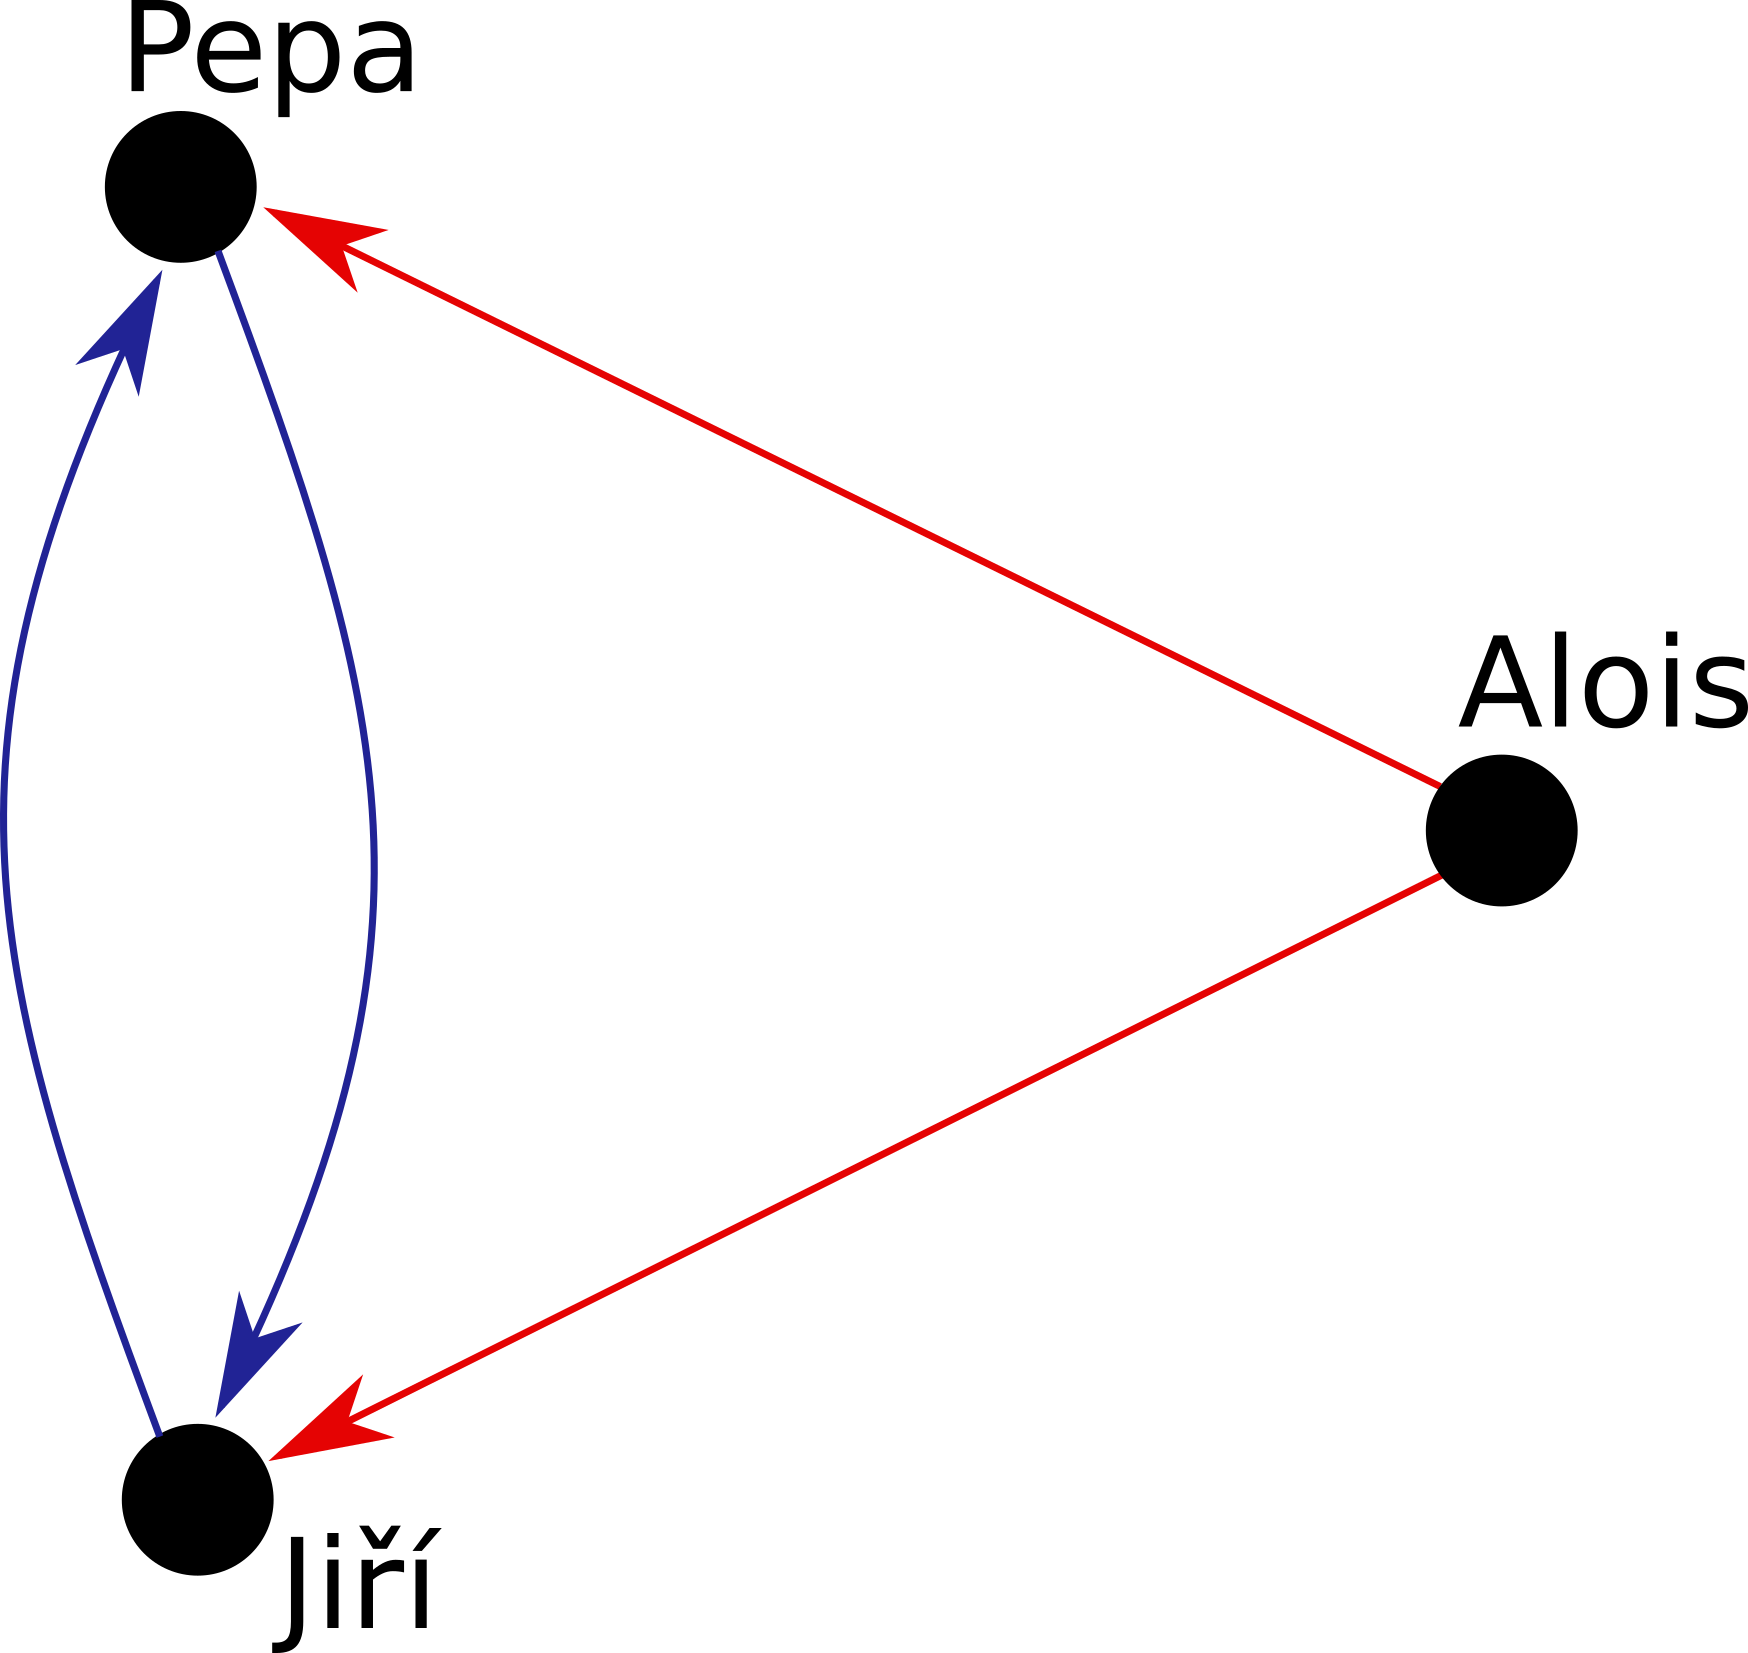
\includegraphics[scale=0.35]{./Pics/pepa.png}
    \caption{Znázorněné šipky směrem k vcholu \textit{Pepa} ukazují ostatní uživatele, jimiž je \textit{Pepa} ovlivněn. Je tedy patrné, že \textit{Pepa} a~      \textit{Jiří} vidí své příspěvky navzájem a~navíc vidí i~příspěvky \textit{Aloisovi}. \textit{Alois} však nevidí ani příspěvky \textit{Pepy}, ani \textit{Jiřího}, neboť příspěvky od těchto dvou uživatelů neproudí směrem k \textit{Aloisovi}.}
\label{fig:pepa}
\end{figure}

Takovouto strukturu můžeme chápat jako orientovaný graf, kde vrcholy před\-sta\-vu\-jí uživatelé \textit{Twitteru} a~orientované hrany mezi nimi proud příspěvků, tedy vztah \textit{following}, neboli \textit{sledující}. Pokud uživatele sleduje mnoho lidí, je směrem k němu připojeno více hran, mluvíme o~uživateli s vysokou konektivitou nebo s vysokým stupněm. Obdobně uživatel, který má malou konektivitu, je takový, k němuž směřuje málo hran, je málo \textit{sledován}.

Příspěvky na \textit{Twitteru} mohou mít jakýkoliv textový tvar do délky $140$ znaků, doplněný obrázkem nebo videem, mnohdy také hypertextovým odkazem na externí článek. Obrázky, videa, ani články na jiných stránkách nejsme schopni analyzovat. Plně však zkoumáme textovou část příspěvků. Ty bývají doplněné o~tzv. \textit{hashtagy}. To jsou slova nebo krátká spojení slov, před kterými stojí znak \textit{\#~(křížek)}. Z pravidla se jedná o~slova, která jsou velmi aktuální, například různé reference na současné politické dění a~podobně. Mnohdy jsou \textit{hashtagy} užívány pouze pro zvětšení popularity příspěvku, jelikož častá forma vyhledávání je právě pomocí \textit{hashtagů}.

\subsection{Data z Twitteru}
\noindent Právě data z \textit{Twitteru} jsou pro nás velmi vhodná. Jak se ukazuje~\cite{whyNotFb}, narozdíl od \textit{Facebooku}, Twitter užívá mnoho uživatelů jako zdroj informací a~zpráv o~ak\-tu\-ál\-ním dění ve světě. Samozřejmě můžeme zpochybňovat validitu a~přesnost informací, které se na takovýchto sítích objevují. Ať už jsou takovéto obavy oprávněné nebo ne, výzkum sociologických jevů, který v této práci provádíme, to nijak neovlivňuje.

Dalším důležitým důvodem, který vedl k výběru Twitteru jako média, ze kterého budeme stahovat informace, je snadná přístupnost k datům pomocí služby API poskytované přímo Twitterem~\cite{twitterAPI}. Konkrétně pro naše účely jsme tuto službu nepoužívali přímo, ale za pomocí balíčku \textit{tweepy}~\cite{tweepy} pro programovací jazyk \textit{python}. Ten umožňuje velmi snadné ovládání a~filtrování proudu dat, které si vyžádáme z Twitteru a~také jejich okamžitou analýzu a~zpracování v \textit{pythonu}.

\subsection{Sentimentální analýza textu}
\noindent Jednou z velice rozvinutých oblastí machine learningu, je tzv. \textit{sentimentální a\-na\-lý\-za textu}, což je forma zpracování přirozeného jazyka\footnote{Pro pojem zpracování přirozeného jazyka budeme užívat převážně zkratku NLP z anglického názvu \textit{Natural Language Processing}}~\cite{NLTKbook}. V základní a~nejvíce studované verzi tohoto problému se snažíme naučit počítač odhadnout, jestli je věta \textit{positivní či negativní}. Existují samozřejmě i~obdobné úlohy. Můžeme se zajímat o~rozdíl mezi větami psanými \textit{objektivně a~subjektivně}, nebo rozlišovat více než dvě kategorie, například rozlišovat texty napsané \textit{rozčíleně, smutně, radostně a~překvapeně}. Záleží pouze za jakým účelem problém řešíme a~datech, které máme k dispozici.

Sentimentální analýza textu se skládá z několika základních kroků, které jsou v obecném měřítku velmi podobné jiným machine learning algoritmům. Základem jsou data. V našem konkrétním případě se jedná přibližně o~$1.5$ miliónů tweetů\footnote{Uspořádaných ve velkém datasetu složeném z několika menších~\cite{TwitterData1, TwitterData2}.} v anglickém jazyce, které jsou označeny lidmi jako positivní, nebo negativní. Algoritmus, který používáme, je neuronová síť~\cite{TwitterSentAnalysis} obohacená o~takzvané \textit{word embedding} vrstvy a~\textit{convolution} vrstvy. Takovýto model je nejdříve \textit{"natrénován"}\footnote{Tréninkem je v této oblasti většinou myšlena optimalizace vhodně zvolené fuknce, která odráží přesnost modelu.} na označených datech\footnote{Data, u kterých označil jejich sentiment reálný člověk, považujeme za správná. i~to je však relativní. Necháme-li více lidí ohodnotit ta stejná data, zjistíme, že ani lidé nejsou v hodnocení příliš konzistetní~\cite{HumanVsMachineLearning}. Pro naše účely je to však naprosto dostačující.}. Poté je možné ho snadno a~s mnohem nižší časovou komplexitou, než byla zapotřebí při tréninku, používat pro predikci sentimentu z textu. Výstupem takového modelu je pravděpodobnost, že předložený text je positivní, tedy reálné číslo mezi $0.0$ a~$1.0$. Takové číslo můžeme chápat jako míru positivity sentimentu textu. Tedy je-li tweet ohodnocen číslem $0.0$, je zřejmé, že je negativní. Je-li ohodnocen číslem $0.5$, chápeme ho jako neutrální. Text ohodnocený číslem $1.0$ je jistě positivní.

Pokud řekneme, že při měření bylo zjištěno, že za určitou dobu bylo v určité skupině $40~\%$ lidí proti a~$60~\%$ pro, je tím myšleno, že $40~\%$ tweetů mělo sentiment menší než $0.5$ a~naopak $60~\%$ větší než $0.5$.

\subsection{Technické detaily sentimentální analýzy textu}
\noindent Pohlédneme-li do větších detailů našeho modelu na odhad sentimentu, prvním krokem po získání datasetu je vytvořit slovník s $V = 5000$ nejčastějšími slovy. Poté je každý datový bod, tedy každý \textit{tweet}, transformován ze seznamu slov do seznamu \textit{1-hot-encoding} vektorů\footnote{Kde každý vektro je reprezantací jednoho slova. Takové reprezantace mají velmi jednoduchý a~zároveň velmi nepraktický tvar. Je-li slovo ve slovníku na $k$-té pozici, bude jeho \textit{1-hot-encoding} reprezentací vektor plný nul, až na $k$-tou pozici, kde se bude nacházet číslo $1$. Každé slovo je tedy reprezentováno vektorem s dimenzí $5000$. Je zřejmé, že tato reprezentace není příliš efektivní.}.

Následuje \textit{word embedding} vrstva~\cite{WordEmbedding1, WordEmbedding2}, která vytvoří novou reprezentaci slov. Ta je schopná mnohem lépe zachovávat semantické vlastnosti jednotlivých slov\footnote{Na takové reprezentaci slov můžeme sledovat zachování semantických vlastností a~dokonce i~možnost heuristického užití aritmetiky. Můžeme si všimnout, že například $vec(\textit{France})\nobreak\hspace{.16667em plus .08333em}-\nobreak\hspace{.16667em plus .08333em} vec(\textit{Paris})\,+\,vec(\textit{Italy})\,\approx\,vec(\textit{Rome})$. Takové vlastnosti jsme při užití \textit{1-hot-encoding} pozorovat nemohli.}. Vektory s dimenzí $V = 5000$ transformuje do vektorů s dimenzí $N = 32$, které se mnohem lépe hodí pro zpracování a~sentimentální analýzu, protože lépe reprezentují skutečný význam slov.

Na tuto vrstvu navazuje \textit{convolution} vrstva~\cite{CNN}, která je schopná prozkoumat postavení slov ve větě. Následuje \textit{fully connected} vrstva, která slouží ke správné interpretaci vlastností odvozených neuronovou sítí, ukončená \textit{relu aktivační jednotkou}. Ta se stará o~dodání nelinearity do modelu, což zajišťuje přesnější klasifikaci. Úplně poslední je další plně propojená vrstva zakončená aktivační funkcí \textit{sigmoid}, která se postará o~transformaci na pravděpodobnost, pro snazší budoucí interpretaci.

Zdrojový kód pro sentimentální analýzu byl napsán v programovacím jazyce \textit{pythonu}, za užití balíčků \textit{TensorFlow}~\cite{TensorFlow} a~\textit{Keras}~\cite{keras}.

% ##############################################################################
% ##############################################################################
\newpage
\section{Konstrukce měření}
\noindent Sentimentální analýza textu nám umožňuje automaticky ohodnotit mírou sentimentu u velkého množství textových příspěvků. Výsledkem takového ohodnocení je však pouze reálné číslo mezi nulou a~jedničkou. Proto odtud nevede žádná přímá cesta k měření síly informační bubliny na částech společnosti. % tady by se hodilo shrnout jak to studují ostatní

Uvažujeme-li konkrétního jedince ve společnosti, informační bublina není nijak explicitně závislá na něm samotném. Místo toho je až implicitně závislá na osobách, které tvoří obsah viditelný námi studovaným jedincem. Proto je zřejmé, že budeme-li chtít pozorovat sílu a~efekt informační bubliny na konkrétního jedince, předmětem našeho studia musí být lidé v okolí tohoto jedince. V případě sociálních sítí to musí být konkrétně příspěvky, které tito lidé tvoří.

Jak jsme již zmiňovali v předešlých kapitolách, pro účely našeho výzkumu jsme využili sociální síť \textit{Twitter}. Ta se v poslední době transformuje spíše do podoby informačního kanálu~\cite{whyNotFb}. Neméně důležitý je fakt, že umožňuje poměrně snadný přístup k datům~\cite{tweepy, twitterAPI}.

\subsection{Sběr dat}
\noindent Našim cílem je pozorovat efekty a~sílu informační bubliny na vybrané skupině ve společnosti. V odstavcích výše jsme však shrnuli, proč to není vůbec přímočarý proces.

Abychom vybrali určitou skupinu uživatelů \textit{Twitteru} co nejpřesněji, využijeme existujících stránek, které sdružují příznivce hledané skupiny. Chceme-li například studovat, jak jsou informační bublinou postiženi \textit{biochemici}, vybereme je z lidí, kteří sledují Twitterový profil \textit{Biochemical Society}. Ten se po našem průzkumu Twitteru ukázal jako nejvíce populární účet s tímto tématem, sleduje ho přibližně $15$ tis. lidí. Služby poskytované Twitterem na stahování dat nás bohužel omezují v počtu zkoumaných uživatelů, proto musíme ze všech $15$ tisíc vybrat pouze část. Abychom zajistili náhodnost tohoto procesu, o~výběr podmnožiny se stará jedna část softwaru~\cite{myRepo}, který jsme pro tyto účely vytvořili. Vybraná skupina sledovaných uživatelů je přehledně zobrazena na obrázku~\autoref{fig:sets}.
\begin{figure}[h]\centering
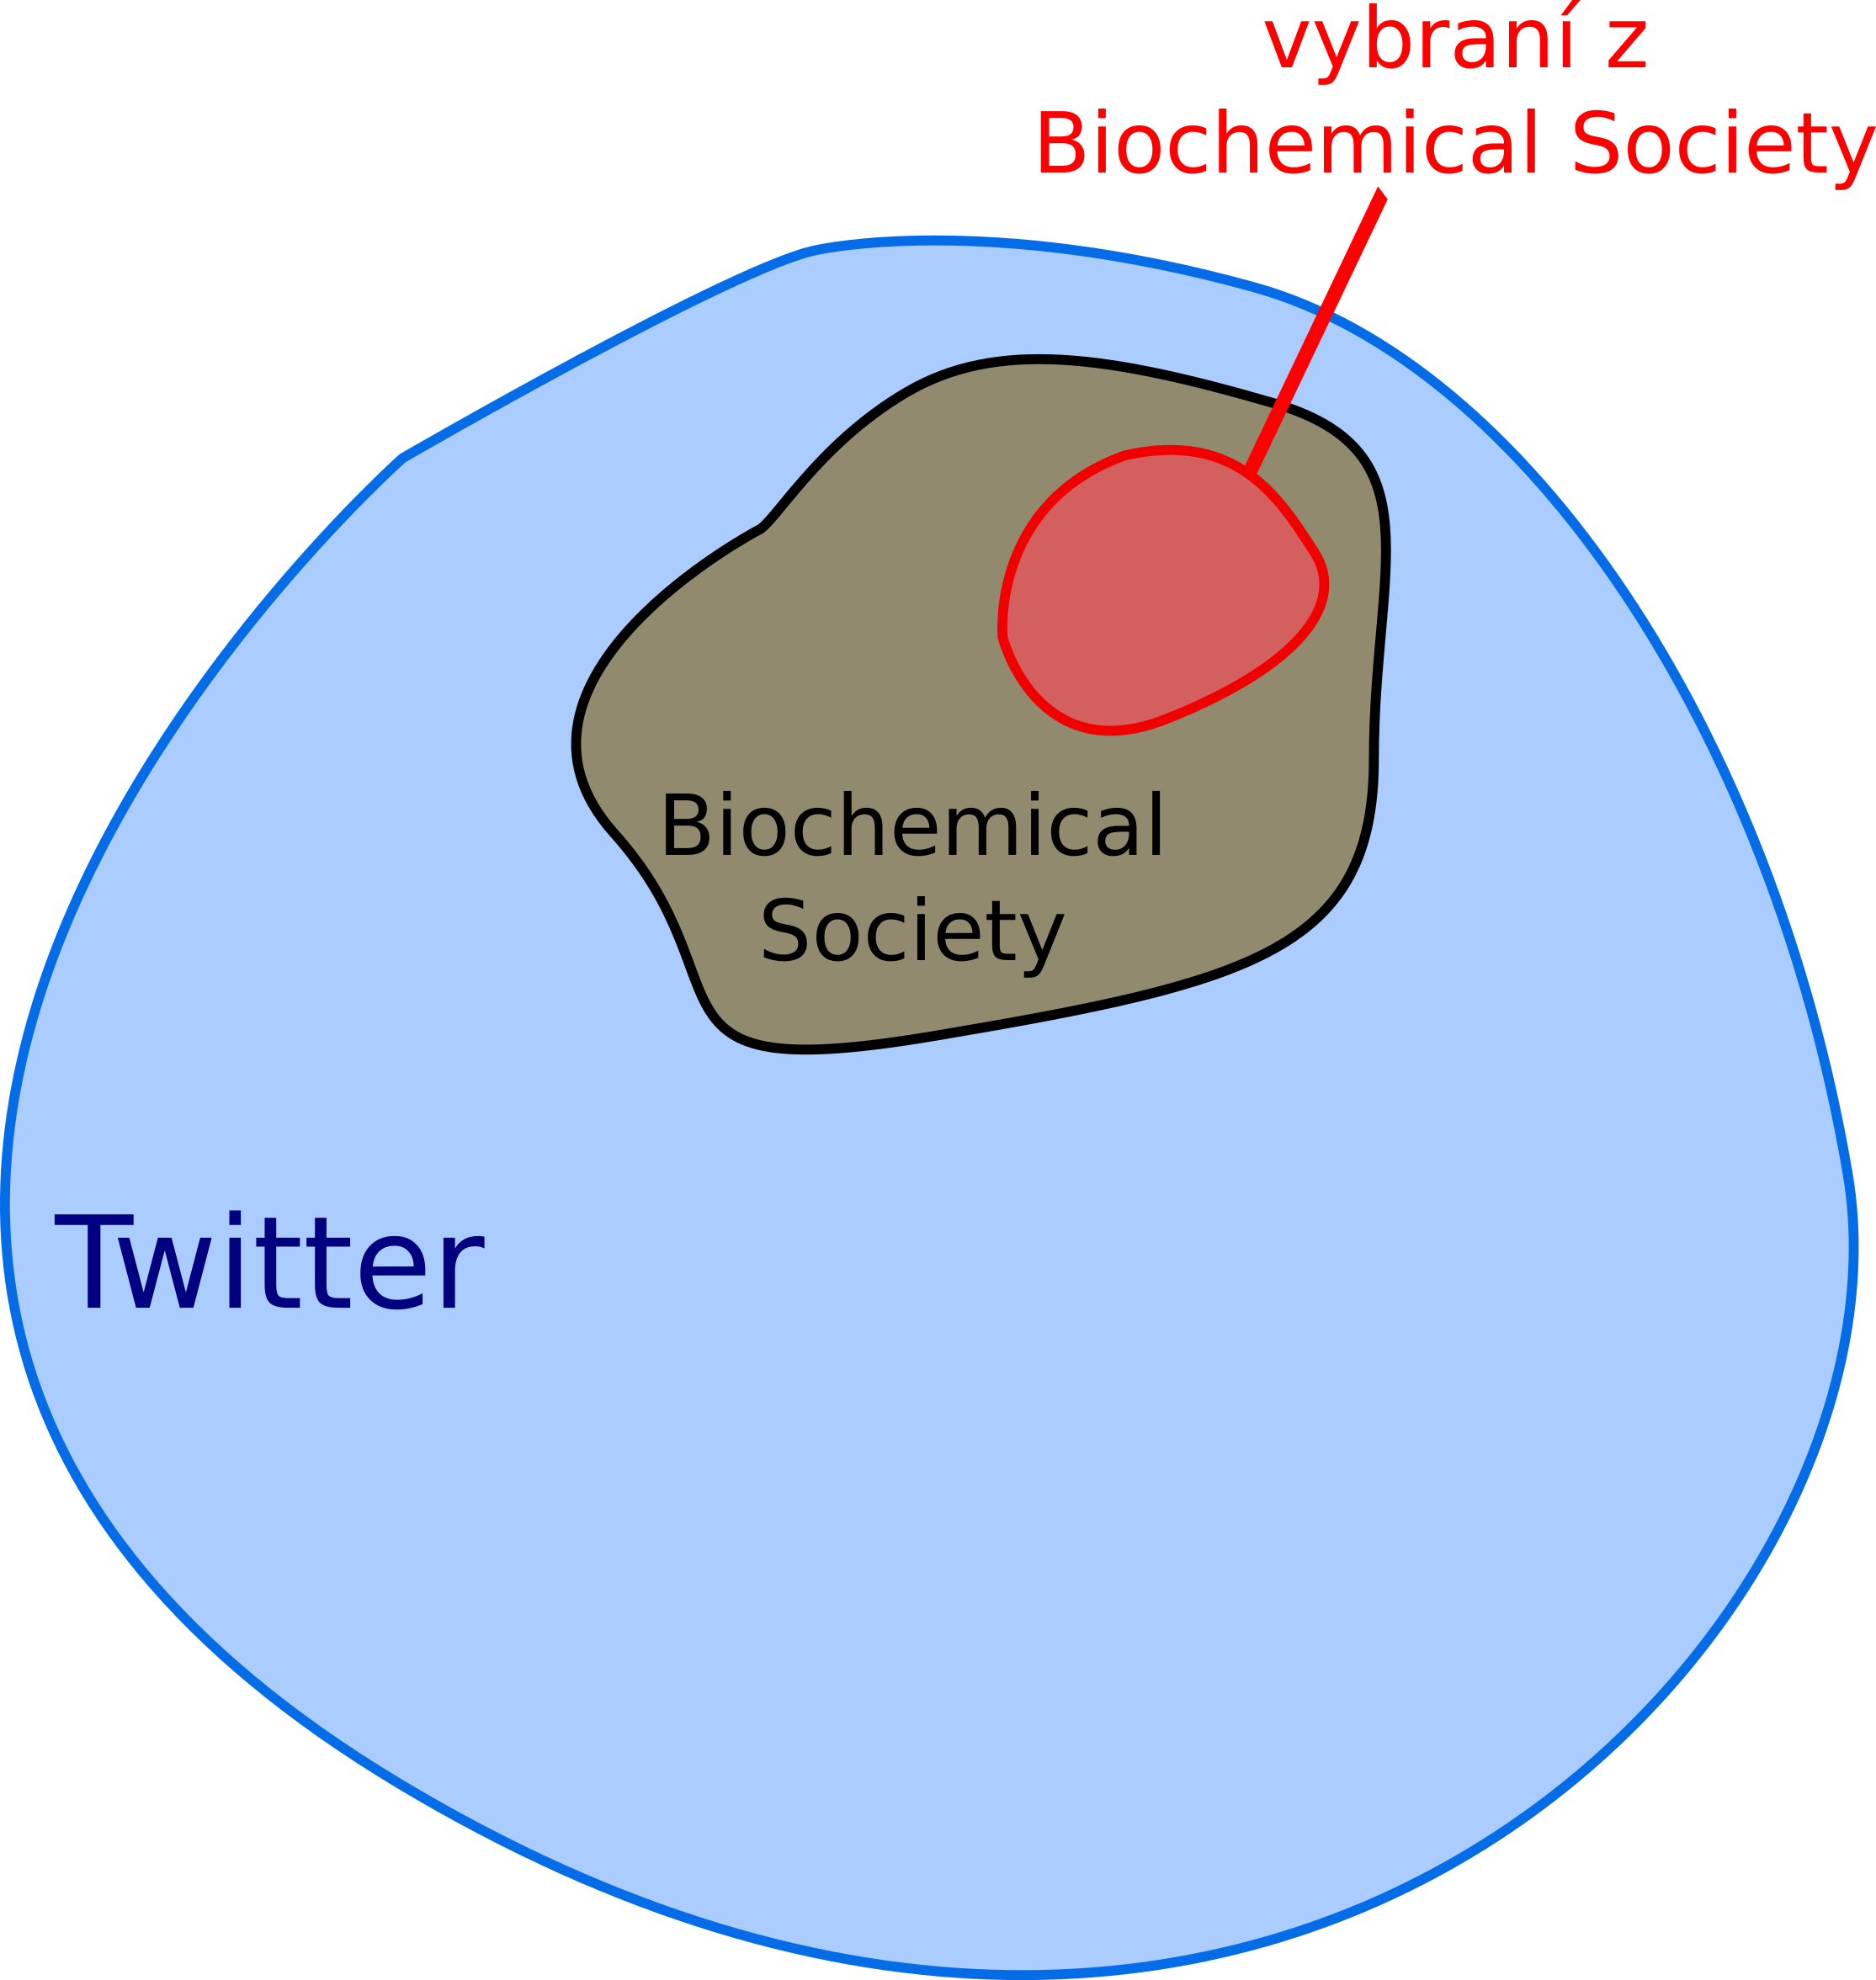
\includegraphics[scale=0.27]{./Pics/sets.png}
    \caption{Twitter vyobrazen jako množina, v níž je znázorněna skupina sledujících \textit{Biochemical Society}. Z této skupiny bylo následně vybráno 100 náhodných uživatelů.}
\label{fig:sets}
\end{figure}

Nyní máme vybranou skupinu vzorků, na kterých chceme pozorovat efekty informační bubliny. Ta je však závislá na uživatelích, kteří vytvářejí obsah vditelný studovanými lidmi. To jsou ti uživatelé, které studované subjekty sledují. Vybereme několik \textit{biochemiků}, na kterých chceme sledovat informační bublinu. Nyní musíme studovat obsah, který tvoří uživatelé sledovaní \textit{biochemiky}. Vztah mezi sledovaným obsahem a~studovanými uživateli je přehledně zobrazen na obrázku~\autoref{fig:followers}.
\begin{figure}[h]
\centering
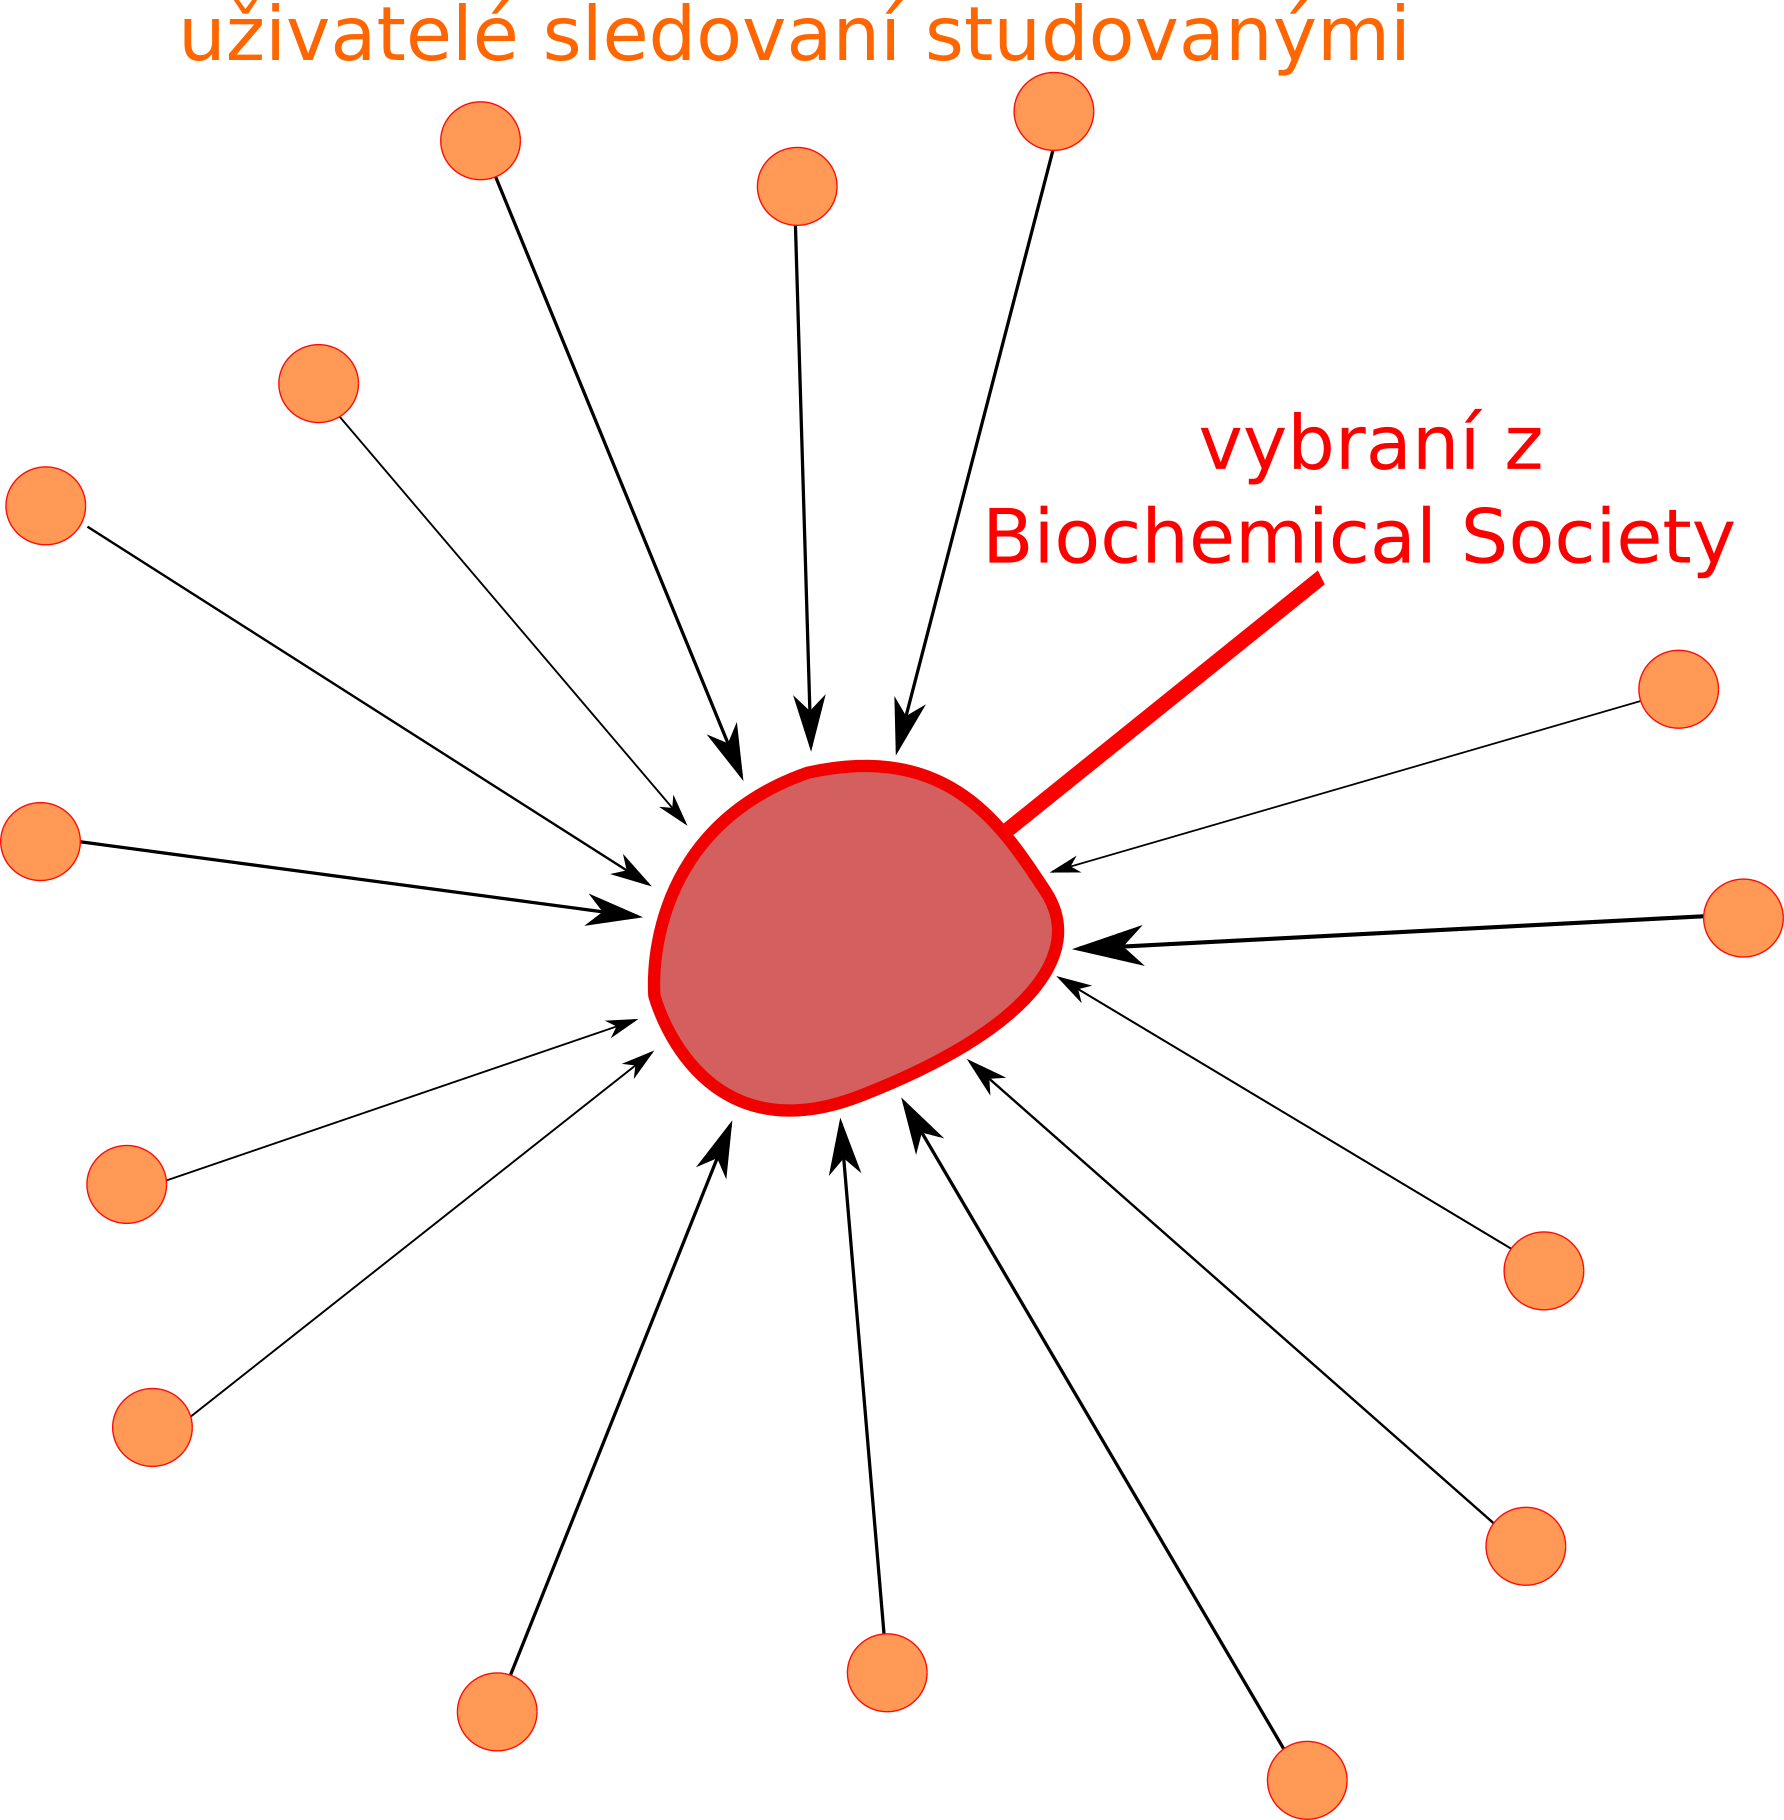
\includegraphics[scale=0.35]{./Pics/followers.png}
    \caption{\textit{Biochemici} znázorněni jako skupina, k níž proudí příspěvky od uživatelů, které sledují. U těchto příspěvků sledujeme diversitu sentimentu jejich obsahu vůči vybraným tématům.}\label{fig:followers}
\end{figure}

Pro přehlednost vyjádřeme tyto vztahy matematicky. Je-li $\mathbb{M}_{bio}$ množina všech uživatelů, kteří sledují stránku \textit{Biochemical Society}, našim prvním úkolem je náhodně vybrat podmnožinu $\mathbb{P}_{bio}$ takovou, že obsahuje námi zvolený počet prvků $\left\vert{\mathbb{P}_{bio}}\right\vert = n$ a~zároveň každý prvek je vybrán s pravděpodobností $p = \frac{1}{\left\vert{\mathbb{M}_{bio}}\right\vert}$. Nyní pomocí služeb poskytovaných Twitterem vybereme množinu $\mathbb{S}_{bio}$ takovou, že každý prvek je sledován alespoň jedním prvkem z $\mathbb{P}_{bio}$. Je-li $\mathbb{T}$ množina všech uživatelů Twitteru a~ $\mathbb{A}$ tzv. \textit{adjacency matrix} celého Twitteru, tedy matice, pro kterou platí:
\begin{equation}
    \mathbb{A}_{ij}=
    \begin{cases}
        1, &\text{pokud j sleduje i;}\\
        0 &\text{jinak.}
    \end{cases}
\end{equation}
Potom $\mathbb{S}_{bio} = \{k\ \text{takové, že}\ \exists l\in\mathbb{T}: \mathbb{A}_{kl} = 1 \wedge l\in\mathbb{P}_{bio} \}$.

\subsection{Pozorování efektů informační bubliny}
\noindent Na takto vybrané skupině lidí $\mathbb{S}_{bio}$, které sledují uživatelé, jejichž informační bublina nás zajímá, chceme pozorovat, zda jsou zaměření pouze jedním směrem a~nepodávají dostatečně široké spektrum názorů. Umíme však pouze odhadnout sentiment jakéhokoliv \textit{tweetu}.

Po dobu měření budeme stahovat všechny tweety, které vytvoří uživatelé z $\mathbb{S}_{bio}$, tedy lidé, které sledují subjekty našeho zájmu. Zajímají-li nás efekty filter bubble na \textit{biochemiky} budeme stahovat všechny tweety, které vytvoří lidé, sledovaní \textit{biochemiky}\footnote{Ve výsledku tedy budeme stahovat všechny tweety, které \textit{biochemici} uvidí, což je právě náš záměr.}.

Ze všech takto stažených tweetů vybereme pouze ty, které obsahují, námi zvolené klíčové slovo. Mohli bychom použít například slovo \textit{\uv{Trump}}. Tím dostaneme pouze tweety, které se zabývají něčím ve vztahu k prezidentu \textit{Trumpovi}. Pro každý takto vyfiltrovaný tweet provedeme sentimentální analýzu a~tím odhadneme, zda má autor positivní nebo negativní vztah k danému tématu. Provedeme-li takováto měření na dvou odlišných skupinách a~stejném klíčovém slově, tedy konkrétním tématu, můžeme odhadovat, kde působí informační bublina. Ať už téma podporuje, či nikoliv. Například můžeme porovnávat rozložení sentimentu zpráv s klíčovým slovem \textit{\uv{Trump}}, které vidí \textit{biochemici} a~příznivci \textit{těžby ropy}. Můžeme předpokládat, že biochemici budou žít v bublině, která má více negativní názor na prezidenta \textit{Trumpa} a~příznivci \textit{těžby ropy} naopak.

Člověku se může zdát, že tímto pouze pozorujeme názor, který mají \textit{biochemici} na \textit{Trumpa}. Tak to ale zdaleka není. Ve skutečnosti zkoumáme, jaké zprávy jsou viditelné \textit{biochemiky}. a~právě zprávy nimi viditelné jsou zdrojem informační bubliny, kterou chceme popisovat.

Zde je potřeba podotknout, že skupiny a~klíčová slova se musí volit velmi pečlivě. Vybereme-li klíčové slovo \textit{\uv{Islámský stát}} a~pozorujeme sentiment, může dojít k velkému nedorozumění. Tweet, který hovoří o~činech páchaných \textit{Islámský stát} bude jistě negativní. Problém však nastává v případě, kdy nějaký tweet hovoří například o~vítězství nad \textit{Islámským státem}. Text takového příspěvku se snadno může jevit jako positivní\footnote{To však není problémem počítače, který text analyzuje. i~člověk by radostný tweet o~vítězství označil jako positivní.}, což bychom špatně vyhodnotili jako tweet podporující \textit{Islámský stát}. Proto je potřeba jak pozorované skupiny, tak klíčová slova volit velmi pečlivě.

V neposlední řadě zmiňme, že data stahovaná z Twitteru jsou již filtrována preferenčními algoritmy. Analyzované příspěvky jsou jen ty, které splňují námi zadané požadavky a~zároveň se objevují na předních pozicích informačních kanálů sledovaných uživatelů\footnote{Vyvstává otázka, jak moc musí být příspěvek sdílený na to, aby byl považován za dostatečně známý a~my ho analyzovali. o~toto se automaticky starají preferenční algoritmy Twitteru~\cite{twitterAPI}, které jsou námi nastavené na úroveň \textit{medium}, což je nejpřísnější nám poskytovaná úroveň filtrace.}. Podotkněme, že toto chování je pro náš výzkum velmi úžitečné, ne-li klíčové. Pokud bychom stahovali všechny příspěvky, i~ty, které se objeví až ve velmi spodní části informačních kanálů, kde je již uživatel nemá šanci zaznamenat, nemohli bychom informační bublinu studovat.

V souvislosti s tímto vyvstává ještě jedna záležitost, která by mohla být zdrojem nedorozumění. Pro kvalitní vysvětlení, předběhněme strukturu naší práce a~uveďme příklad. Jednou z pozorovaných skupin je skupina \textit{feministek} s klíčovým slovem \textit{\uv{abortion}}. Porovnáme-li analyzovaná data této skupiny s daty s příspěvky z celého \textit{Twitteru}\footnote{Tedy s příspěvky, které nejsou nijak omezeni skupinou, která je vidí.} zjistíme, že tweetů viditelných \textit{feministkami} je podstatně více než tweetů viditelných celým \textit{Twitterem}. Co se může zdát naprosto nesmyslné. Vždyť skupina \textit{feministek} je jistě podmnožina celého \textit{Twitteru}, proto by počet příspěvků s daným klíčovým slovem měl být podstatně menší. Ve skutečnosti nám však toto říká, že počet často sdílených příspěvků s daným klíčovým slovem je větší u \textit{feministek} než u náhodného uživatele \textit{Twitteru}.

\subsection{Výběr pozorovaných skupin}
\noindent Pro naše měření jsme provedli důkladný výběr studovaných objektů vycházející z nejaktuálnějšího politického dění, abychom dosáhli co nejpřesnějšího zachycení veškerých možných skupin názorů.

Z důvodu fungování naší metody v anglickém jazyce jsme nevolili témata lokální, kupříkladu z české politické sféry, jež by svým rozsahem a~především jazykem nevyhovovala měření, nýbrž jsme zvolili témata globálního rozsahu řešící se na sociálních sítích zejména v anglickém jazyce.

Jako velmi rozporuplnou a~politicky zajímavou veřejně známou osobností jsme vybrali nedávno zvoleného prezidenta Spojených států amerických Donalda Trumpa. Nynější prezident Trump byl již ve své předvolební kampani zastáncem radikálních změn, heslo \uv{Make America Great Again} a~příslib zlepšení finanční situace musel velice imponovat nižší a~střední třídě společnosti. Z tohoto důvodu se nám společnost \textit{příznivců těžby ropy} zdála být optimální volbou.

Jak se také Trump ve svých výrocích zmínil, hodlá snížit dotace na rozvoj vědy, proto usuzujeme, že právě vědecká společnost \textit{biochemiků} bude mít názor na prezidenta Trumpa poněkud negativnější než názor příznivců \textit{těžby ropy}. U těchto dvou skupin jsme proto vybrali jako klíčové slovo heslo \textit{\uv{Trump}}.

Námi druhé zvolené heslo \textit{\uv{abortion}}\footnote{Slovo, jež v angličtině znamená \textit{\uv{potrat}}.} má také co dočinění s americkou politickou sférou. Trump se jako silný republikán s přáním stále rostoucího počtu amerických obyvatel vyjádřil velmi negativně o~problematice potratu. Zmínil se o~celoplošném zákazu potratů v USA, což vzbudilo v obyvatelstvu silné emoce, a~to jak positivní, tak negativní.

Velký potenciál, co se týče příznivců potratů, jsme spatřovali v organizaci \textit{Guttmacher Institute} podporující vzdělání, ochranu a stejné možnosti žen a můžů ve zdravotní péči. Další skupinu příznivců jsme identifikovali jako \textit{Planned Parenthood}. Hlavním cílem tétéo organizace je ochrana jak právní, tak i zdravotní bez ohledu na finance daných osob, převážně žen v těžkých situacích.  Třetí námi sledovanou výraznou komunitou byla feministická skupina \textit{Everyday Feminism}, jež tradičně podporuje rovnoprávnost žen ve všech oblastech společnosti.

Na rozdíl od těchto dvou podskupin potenciálních sympatizantů s potraty jsme vyhledali skupiny lidí s odlišnými etickými zásadami. Pro tyto účely byla zvolena komunita \textit{Abolish Abortion USA}, která se zastává pozměnění ústavy, tedy zákazu potratů. Druhá skupina~\textit{Students fo Life}, orientující se spíše proti potratům, se snaží o sexuální vzdělání mladých lidí pomocí přednáškových cyklů.  

U těchto dvou skupin bychom mohli očekávat výsledky na téma potrat výrazněji odlišné, než u předchozích tří.

% ##############################################################################
% ##############################################################################
\newpage
\section{Diskuze měření}
\noindent Pozorované skupiny jsme vybírali tak, abychom mohli pozorovat co nejsilnější efekty informační bubliny. Sledované komunity se tedy liší názorem na dané pozorované téma.  Je klíčové pochopit, že našim cílem není ukázat to, že mají jiný názor. Cílem je prezentovat rozdílnost v příspěvcích, které na sociální sítí členové komunit vidí. Pomocí našich výsledků poté okomentovat jak moc je ohrožena objektivita uživatelů sociálních sítí.

\subsection{Klíčové slovo: potrat}\label{subsec:abortion}
\noindent Začněme s případem, kdy jsme se zabývali diversitou názorů na \textit{\uv{potrat}}. Hledali jsme příspěvky s klíčovým slovem \textit{\uv{abortion}} a~sledovali, zda se sentiment takovýchto příspevků liší v různých skupinách\footnote{Konkrétně šlo o~\textit{katolíky} sledující skupinu \textit{Catholic News Svc}, \textit{mormony} sledující skupinu \textit{Only Mormons}, \textit{feministky} sledující skupinu \textit{Everyday Feminism} a~uživatele sledující skupinu \textit{LGBT foundation}.}. Předpokládali jsme, že \textit{katolíci} a~\textit{mormoni} budou spíše proti potratům, jejich sentiment bude tedy spíše nižší. Narozdíl od toho u \textit{feministek} a~uživatelů sledujících \textit{LGBT foundation} jsme očekávali vyšší sentiment. Tyto skupiny jsme následně porovnávali i~se sentimentem a~frekvencí příspěvků s tímto klíčovým slovem na celém \textit{Twitteru}\footnote{Takto vybrané příspěvky můžeme v jístém smyslu považovat za průměrný názor uživatelů \textit{Twitteru} a~vůči nim následně porovnávat efekty informační bubliny v jiných skupinách.}.
\begin{figure}[!h]
\centering
\subfloat[Všechny skupiny krom \textit{Everyday Feminism}.]{\label{fig:abortion-3groups}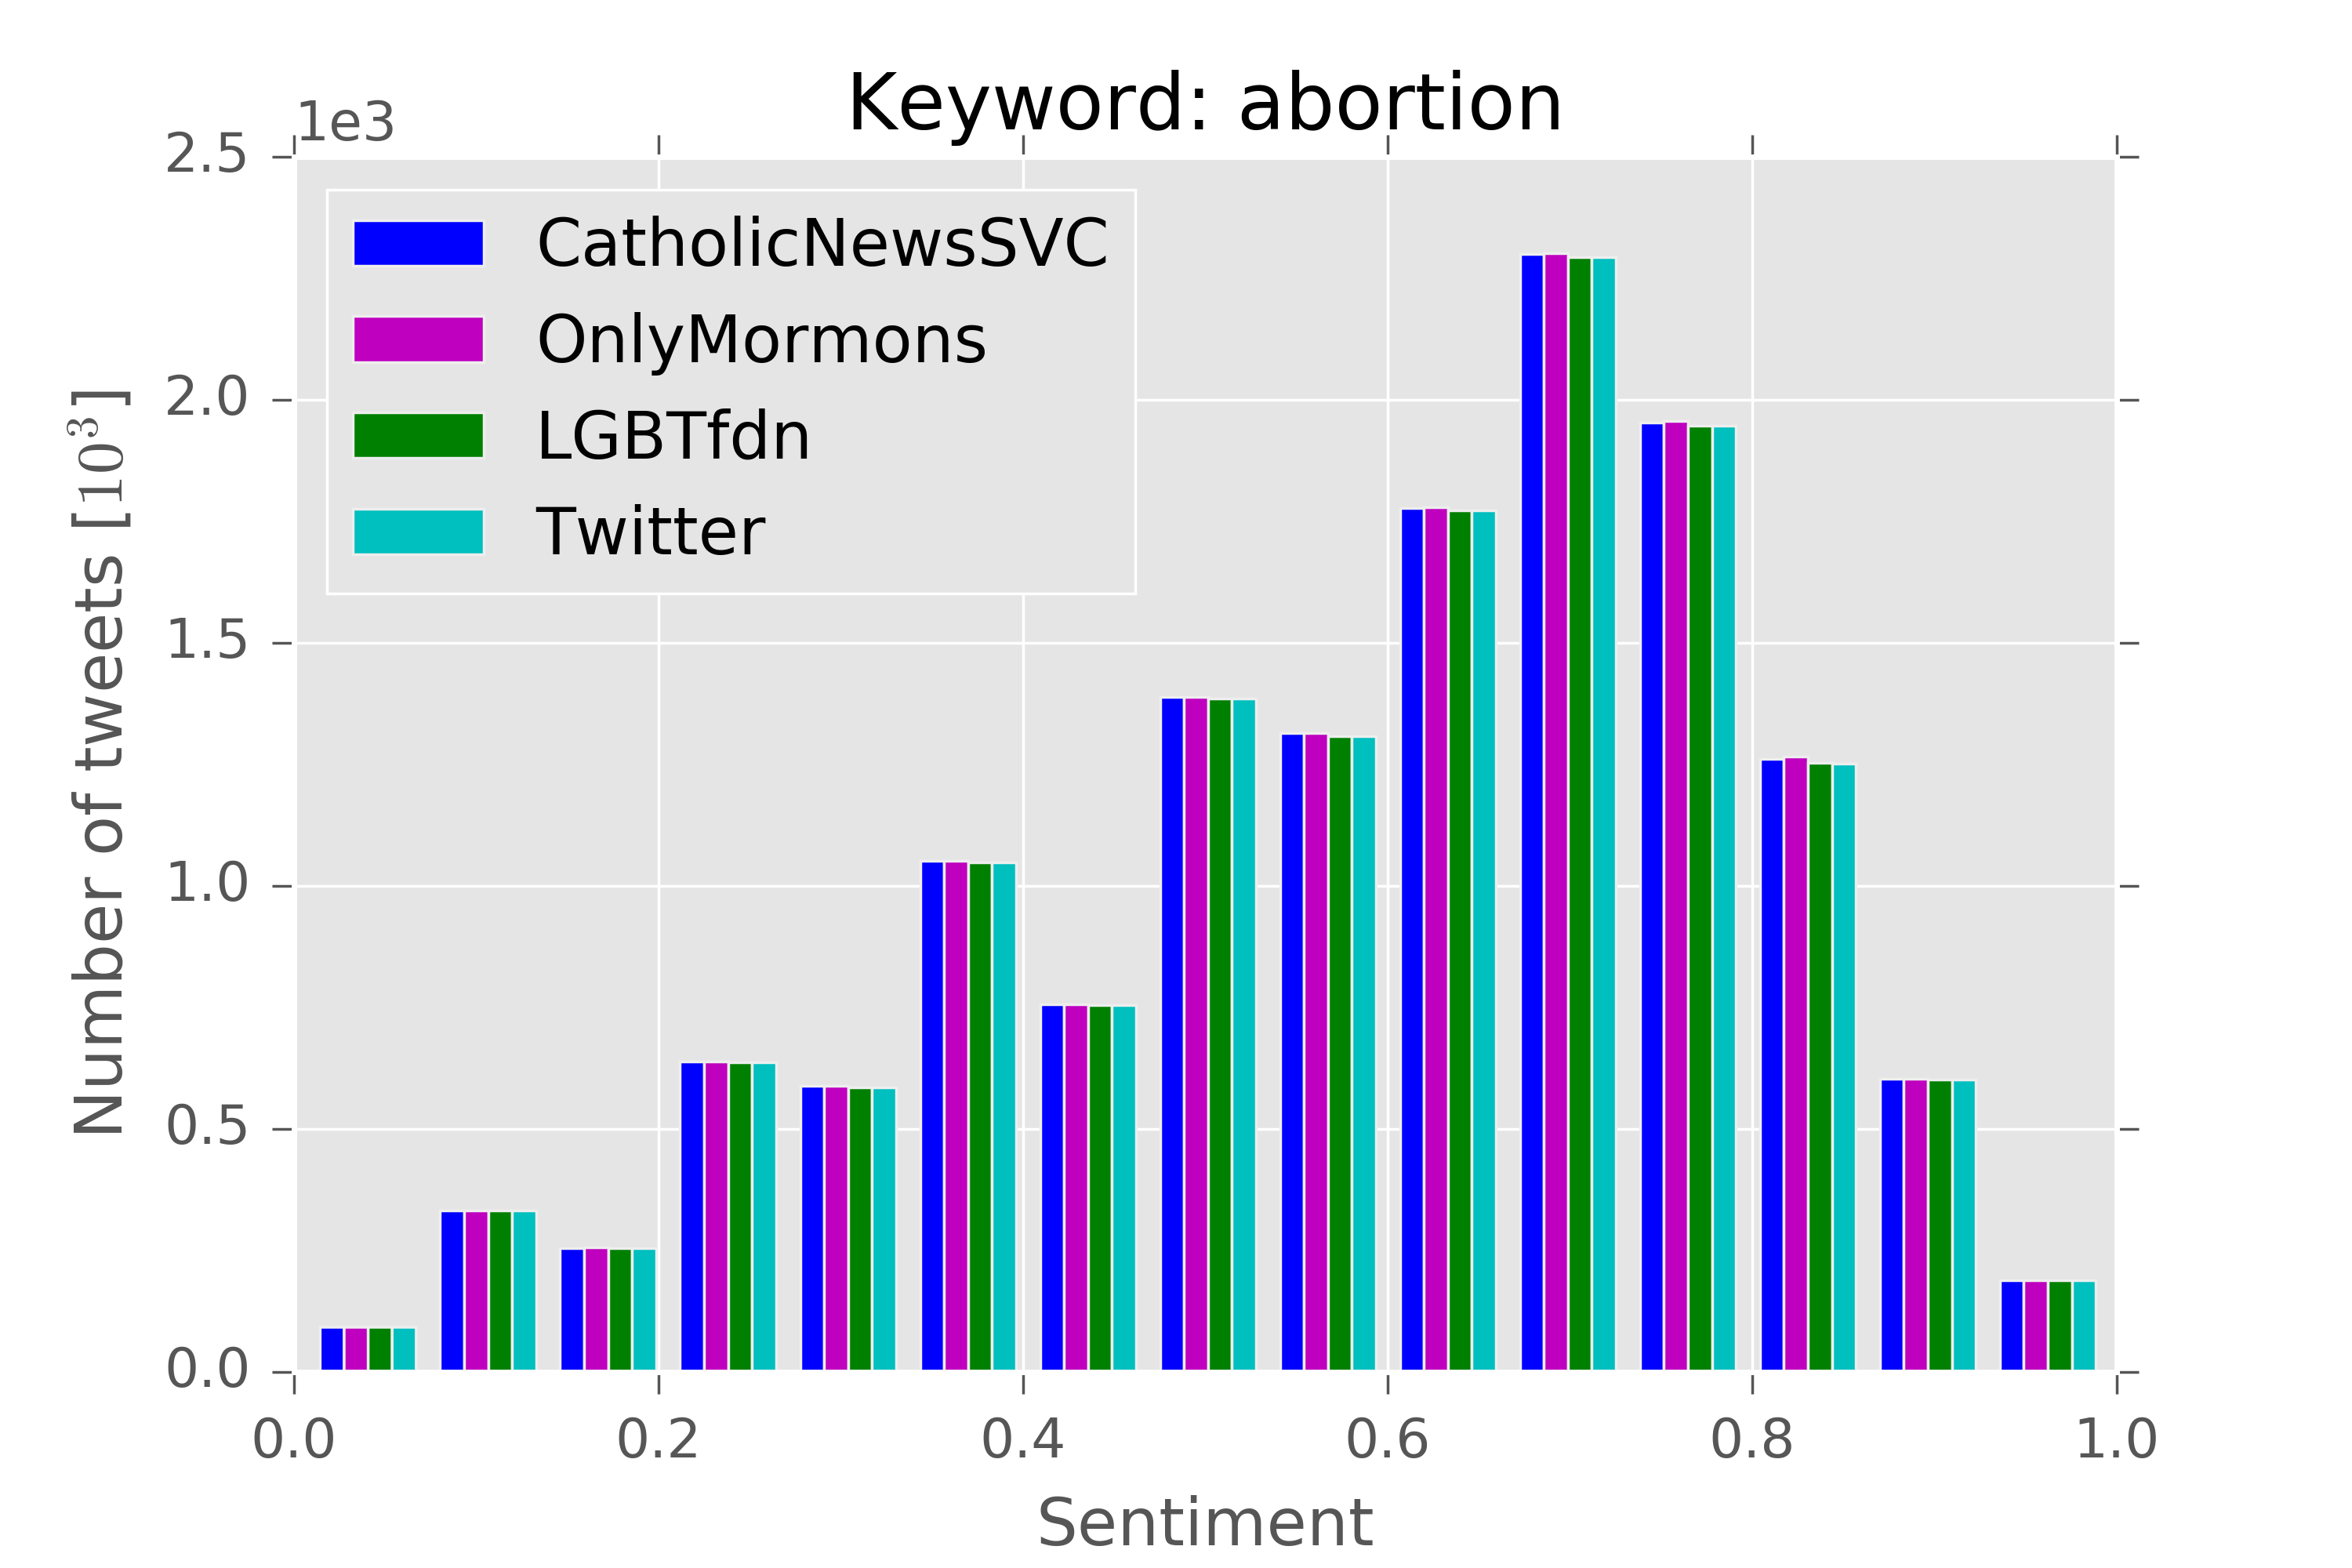
\includegraphics[scale=0.5]{./Pics/abortion-3groups.png}}
\subfloat[\textit{Everyday Feminism} a~\textit{Catholic News Svc}]{\label{fig:feminismXcatholic}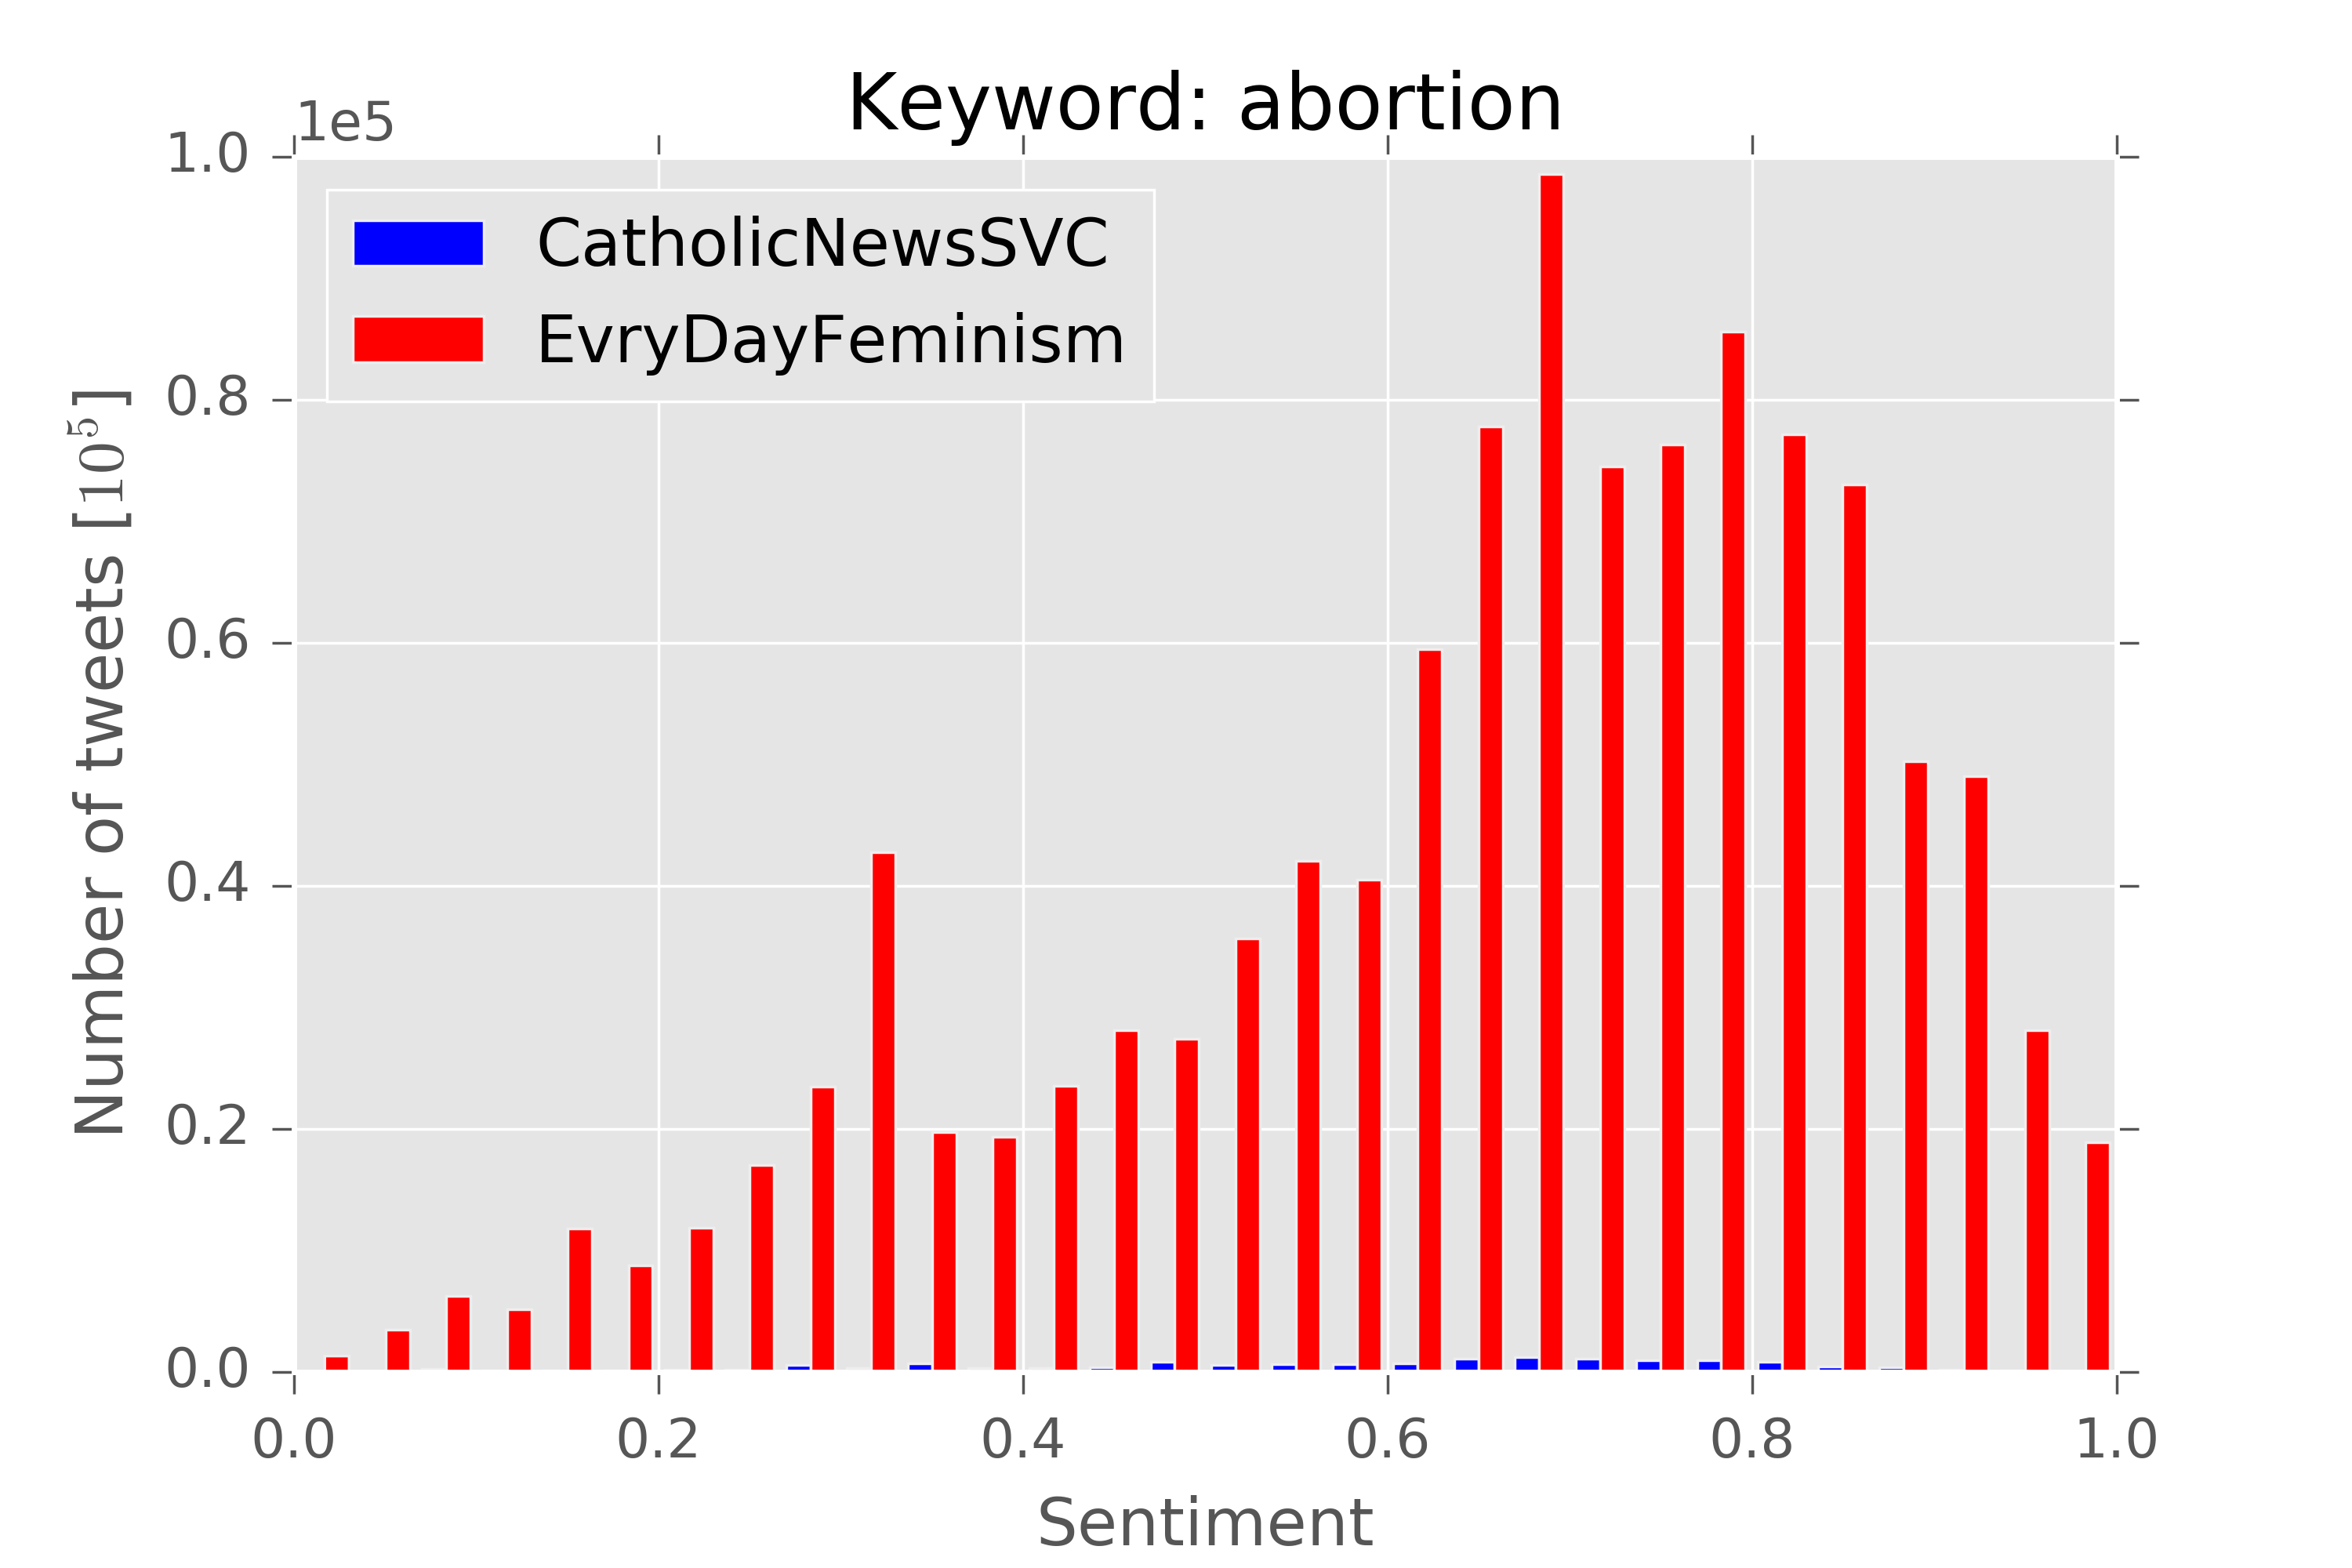
\includegraphics[scale=0.5]{./Pics/feminismXcatholic.png}}
\caption[]{Histogramy počtu tweetů u skupin s klíčovým slovem \textit{\uv{abortion}}.}
\label{fig:abortion1}
\end{figure}

Na obrázcích~\autoref{fig:abortion1} vidíme histogramy\footnote{Na svislé ose je v tomto případě vždy počet příspěvků s příslušnou naměřenou hodnotou sentimentu, která je vyznačena na vodorovné ose. Toto zobrazení nám umožňuje snadno nahlédnout na rozdělení sentimentu v příspěvcích i~na počty příspěvků s daným tématem.} sentimentu příspěvků uvedených skupin. Měření probíhalo v době od 18.03.2017 17:00 do 19.03.2017 08:00.

Překvapivě, z obrázku~\autoref{fig:abortion-3groups} jde vidět, že tři skupiny \textit{Catholic News Svc}, \textit{Only Mormons} a~\textit{LGBT foundation} mají rozdělení identické s náhodným výběrem z celého Twitteru. Rozdělení sentimentu i~počty příspěvků s tímto tématem jsou naprosto shodné. Toto zjištění pro nás bylo poměrně překvapující. Můžeme říct, že komunity \textit{Catholic News Svc}, \textit{Only Mormons} a~\textit{LGBT foundation} se v diskuzi okolo \textit{potratu} dostanou k obsahu, který je v rámci Twitteru absolutně vyvážený.

Na rozdíl od toho, podíváme-li se na histogram~\autoref{fig:feminismXcatholic} zobrazující rozdělení sentimentu u skupin \textit{Catholic News Svc} a~\textit{Everyday Feminism} vidíme obrovský rozdíl\footnote{Rozdíl je ve dvou řádech, proto se může stát, že malé modré sloupce zobrazující počty tweetů skupiny okolo \textit{Catholic News Svc} nejsou dostatečně viditelné.} v samotném počtu často sídlených tweetů s tématem \textit{potratu}. Už tento fakt naznačuje poměrně silnou informační bublinu, ve které jsou pohlceni členové komunity \textit{Everyday Feminism}.
\begin{figure}[h]
\centering
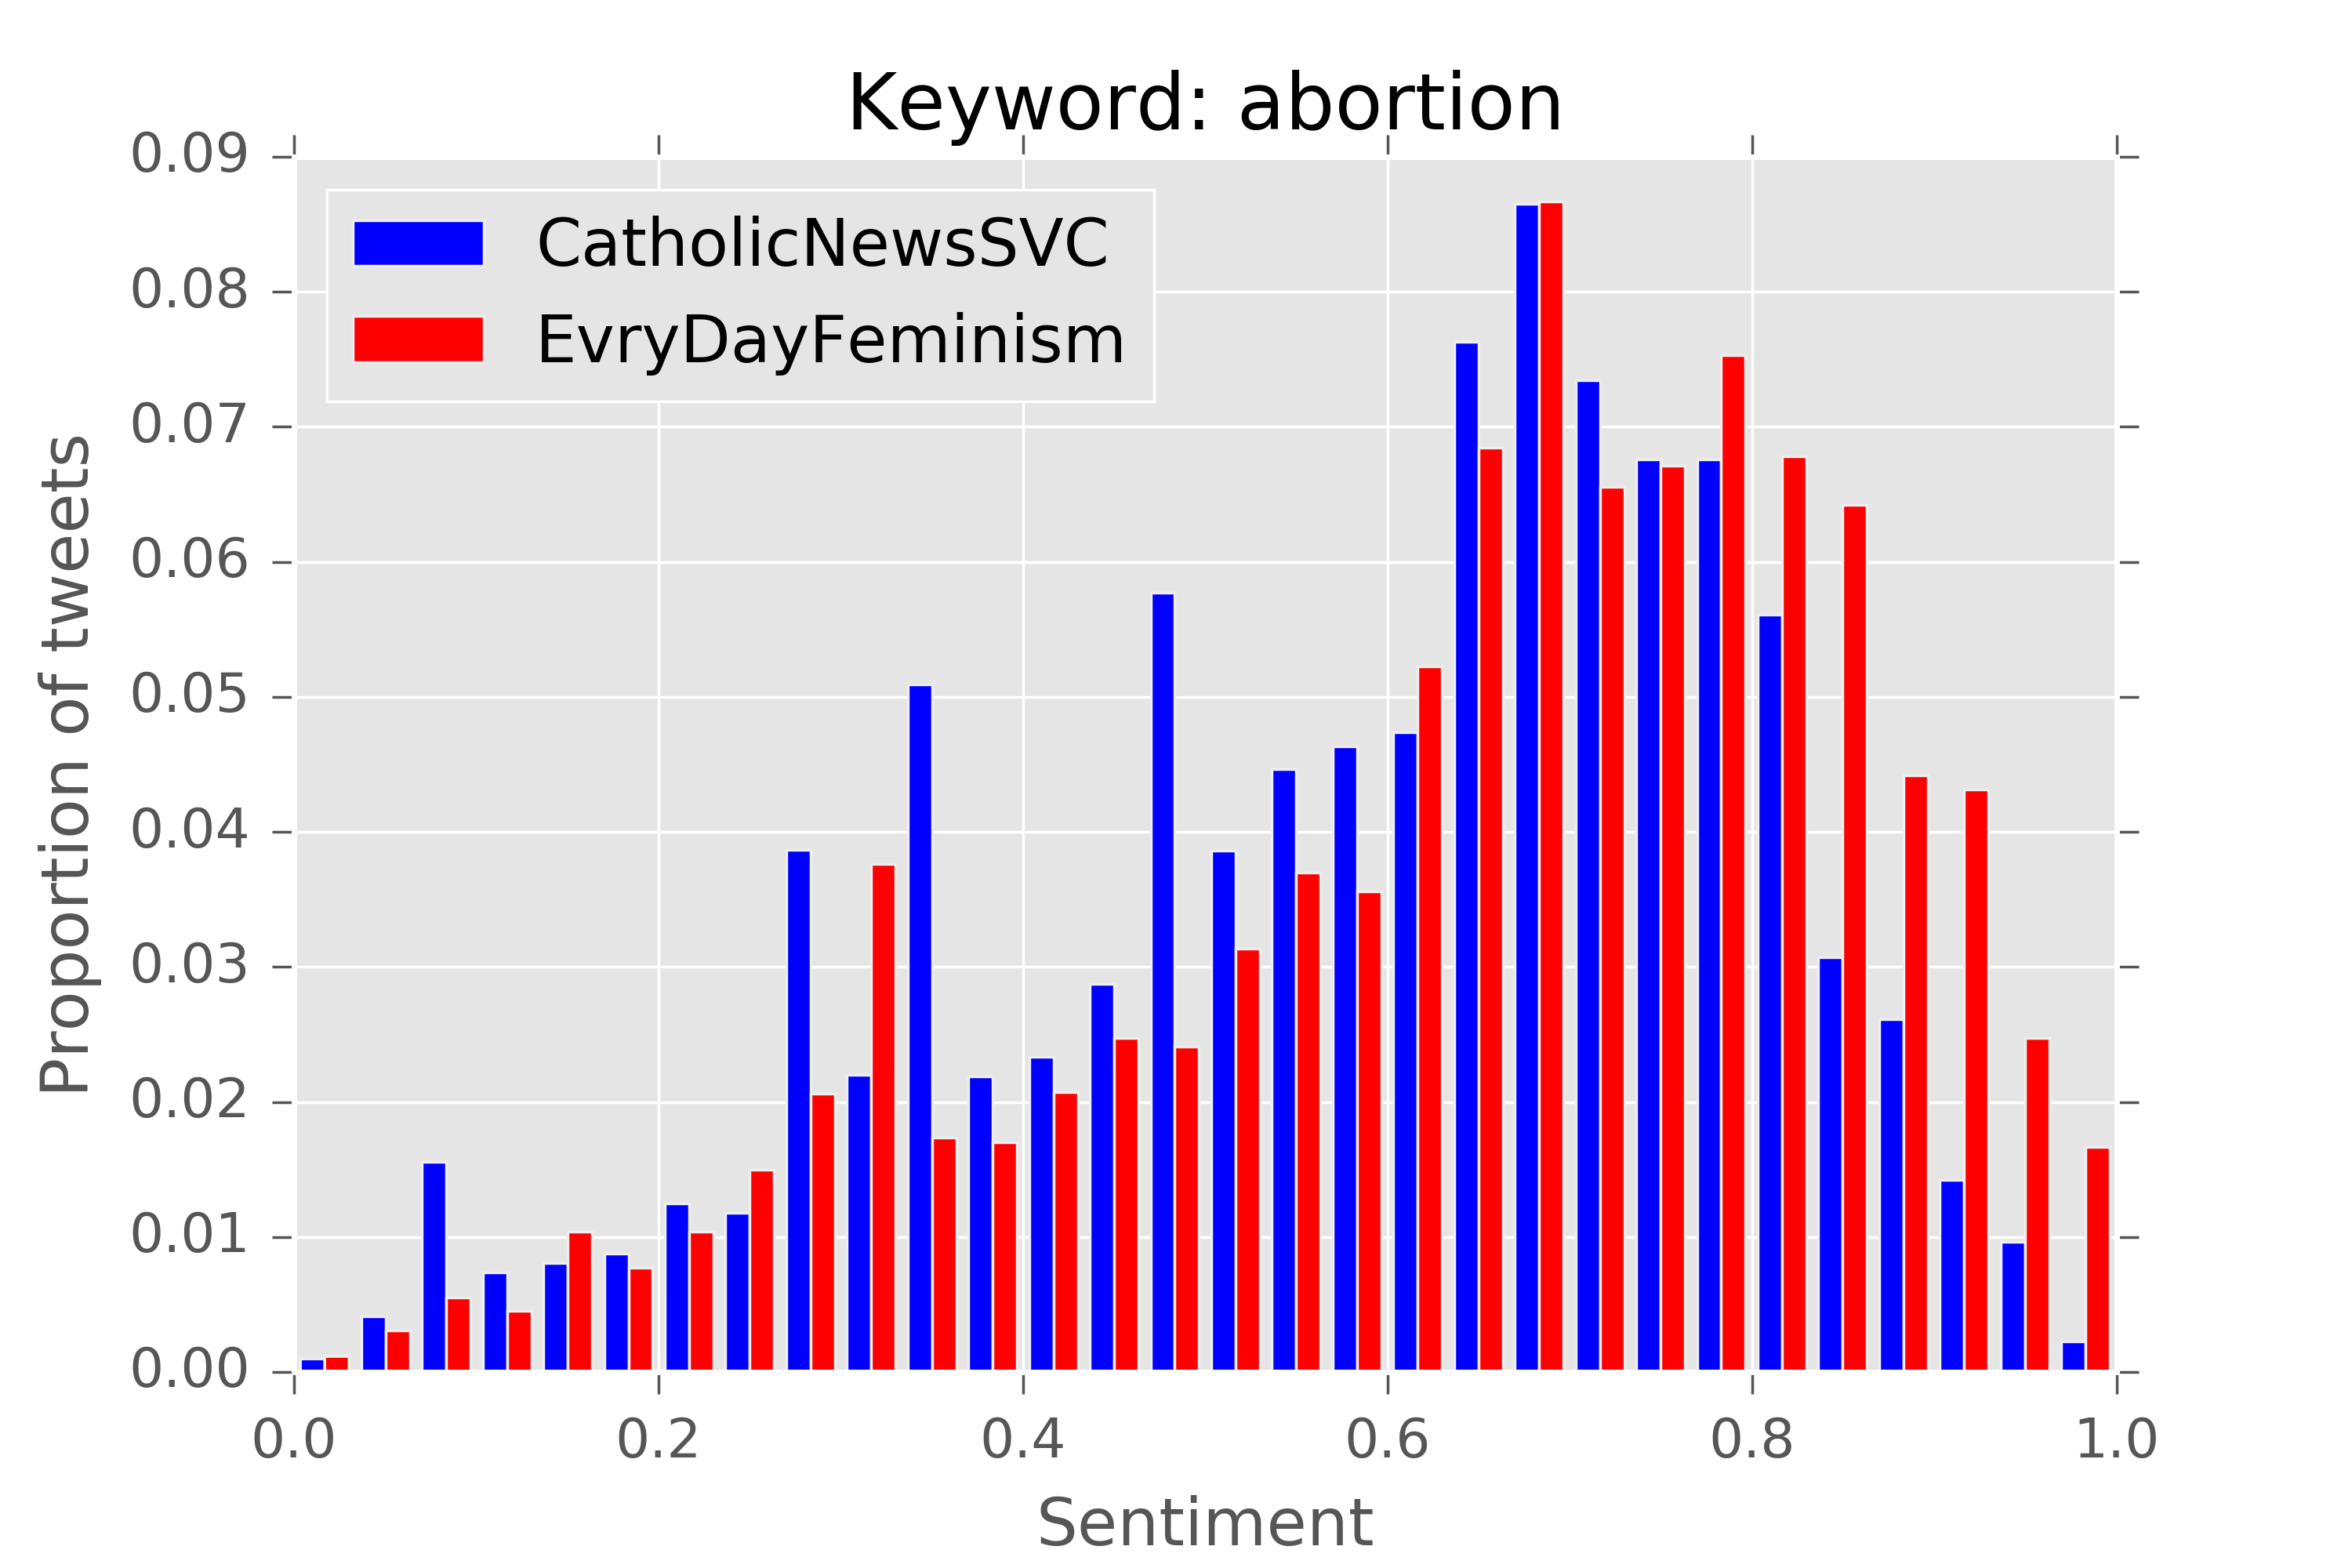
\includegraphics[scale=0.5]{./Pics/feminismXcatholic-normed.png}
\caption{Normalizované rozdělení sentimentu příspěvků, které vidí komunity \textit{Catholic News Svc} a~\textit{Everyday Feminism}.}
\label{fig:feminismXcatholic-normed}
\end{figure}
Abychom mohli prostudovat i~rozložení sentimentu a~nejenom počet příspěvků vztahujících se k danému tématu, pohlédněme na histogram~\autoref{fig:feminismXcatholic-normed}, který zobrazuje normalizované\footnote{V tomto případě se díváme na normalizovaný histogram. Na svislé ose tedy nejsou skutečné počty příspěvků s daným sentimentem vyneseným na vodorovné ose. Místo toho je na svislé ose podíl tweetů s daným sentimentem a~celkovým počtem tweetů ve sledované skupině. Toto zobrazení nám dovoluje studovat rozložení sentimentu dvou skupin, bez ohledu na rozdíl mezi absolutními počty příspěvků.} rozdělení zmíněných dvou skupin.

Při porovnání komunity \textit{Everyday Feminism} a~komunity \textit{Catholic News Svc}, která v daném tématu není nijak postižena informační bublinou je patrný markantní rozdíl. Vidíme, že v levé části, kde jsou hodnoty sentimentu menší než $0.5$ lehce převažují příspěvky, které vidí komunita \textit{Catholic News Svc}. Kdežto v pravé části, kde jsou zobrazeny proporce příspěvků s velmi vysokým sentimentem naprosto jednoznačně převažuje komunita \textit{Everyday Feminism}. Uživatelé sledující \textit{Catholic News Svc} vidí $31~\%$ negativních\footnote{Pod pojmem negativní příspěvek rozumněj takový tweet, který má hodnotu sentimentu menší než $0.5$. Obdobně definujeme i~positivní příspěvek.} příspěvků na téma \textit{potratu} a~$69~\%$ kladných příspěvků. Tyto hodnoty jsou stejné i~pro náhodný výběr z celého Twitteru. Narozdíl od toho uživatelé sledující \textit{Everyday Feminism} vidí $22~\%$ negativních a~$78~\%$ positivních příspěvků.

Z výše prezentovaných výsledků je patrné, že narozdíl od skupin \textit{Catholic News Svc}, \textit{Only Mormons} a~\textit{LGBT foundation} jejichž obsah je v oblasti debaty nad tématem \textit{potratu} naprosto vyvážený, komunita \textit{Everyday Feminism} se k vyváženému obsahu přímo nedostává. Počet a~hlavně rozdělení příspěvků na dané téma se výrazně liší od ostatních skupin i~náhodného výběru z celého Twitteru. Můžeme tedy říct, že je postižena informační bublinou.

Někdo by mohl namítat, že rozdíl nebyl dostatečně markantní. Je však potřeba si uvědomit, že díky velké konektivitě uživatelů Twitteru je alespoň základní přístup k různým názorům snado zajištěn. Při hledání informační bubliny je tedy třeba pozorovat i~zdánlivě malé rozdíly v rozdělení, nebo četnosti určitých příspěvků.
% TODO: rozsirit tento druh povidani?

\subsection{Klíčové slovo: Trump}\label{subsec:Trump}
\noindent Donald Trump, prezident Spojených států amerických, je v dnešní době sám o~sobě velké téma snad všude na světě. Proto byla předmětem několika z našich pozorování.

Nejprve jsme pozorovali, zda se nevyskytuje efekt informační bubliny v komunitě \textit{biochemiků} okolo twitterové skupiny \textit{BiochemSoc} a~lidí zajímajících se o~\textit{těžbu ropy} sdružujících se okolu skupiny \textit{PetroleumEcon}. Měření probíhalo v době od 18.03.2017 10:20 do 18.03.2017 16:00. Dá se předpokládat, že kvůli prohlášením Donalda Trumpa o~vědě a~jeho postojům k těžbě ropy, bude komunita \textit{biochemiků} zahlcována spíše negativními příspěvky, narozdíl od toho komunita okolo \textit{těžby ropy} spíše positivními.

Z histogramu~\autoref{fig:biochem_petroleum-trump} vidíme, že naše očekávání nebyla správná. Počty tweetů u obou skupin, tj. \textit{BiochemSoc}, \textit{PetroleumEcon} a~náhodného výběru z \textit{Twitteru}, jsou řádově naprosto stejné. i~samotné rozdělení sentimentu je totožné. Z výsledku můžeme usuzovat, že komunita okolo \textit{BiochemSoc} je vystavena nepatrně většímu počtu příspěvků na dané téma. Rozdíl je však zanedbatelný.
\begin{figure}[h]
\centering
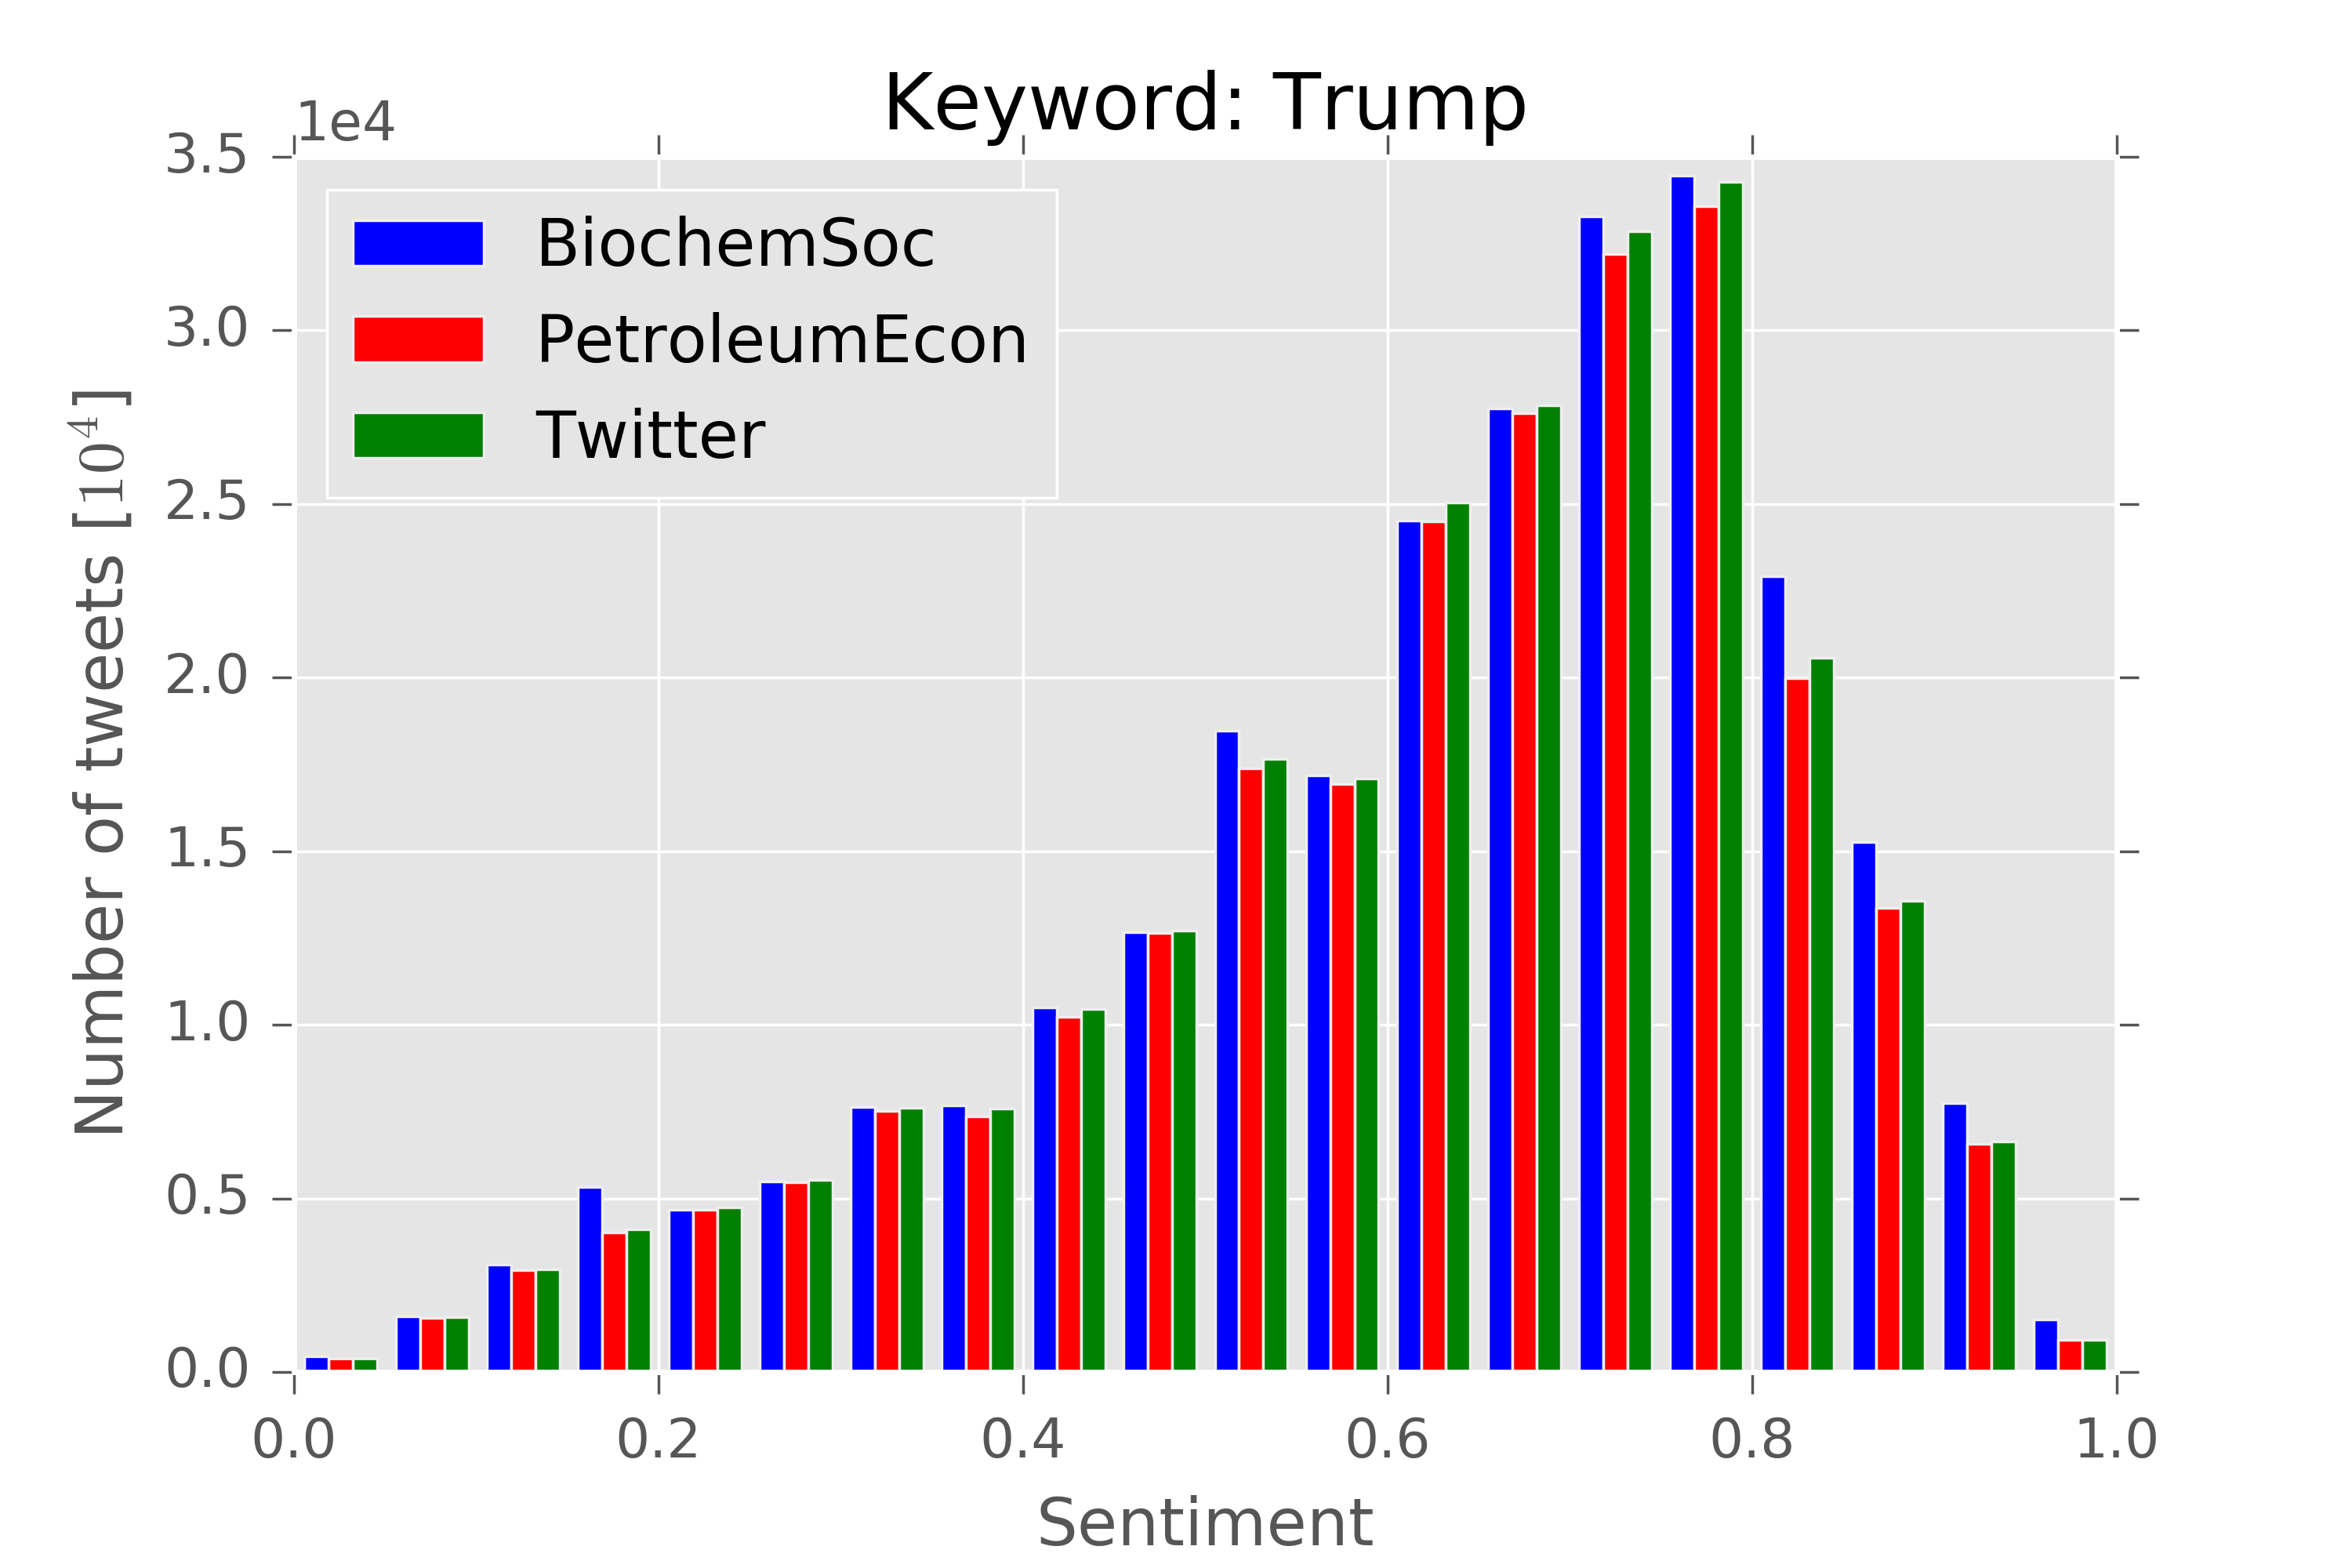
\includegraphics[scale=0.5]{./Pics/biochem_petroleum-trump.png}
\caption{Histogramy počtu tweetů u skupin s klíčovým slovem \textit{\uv{Trump}}.}
\label{fig:biochem_petroleum-trump}
\end{figure}

Narozdíl od našeho očekávání můžeme konstatovat, že skupiny \textit{BiochemSoc} a~\textit{PetroleumEcon} jsou vystaveny dostatečně vyváženému obsahu na dané téma a~nejsou tedy ohroženi informační bublinou. To je pravděpodobně způsobeno velkou konektivitou uživatelů Twitteru, která je spojuje s dostatečně velkým množstvím lidí opačných názorů.

Další skupinou, která by mohla být postižena nedostatečně vyváženým obsahem v tématu \textit{\uv{Trump}} jsou potomci indiánů a~jejich podpůrci. Tuto komunitu jsme identifikovali jako uživatele sledující Twitterovou stránku \textit{StandingRockST}. Porovnávali jsme je s náhodným výběrem z Twitteru. Měření probíhalo v době od 19.03.2017 18:00 do 19.03.2017 22:00.
\begin{figure}[h]
\centering
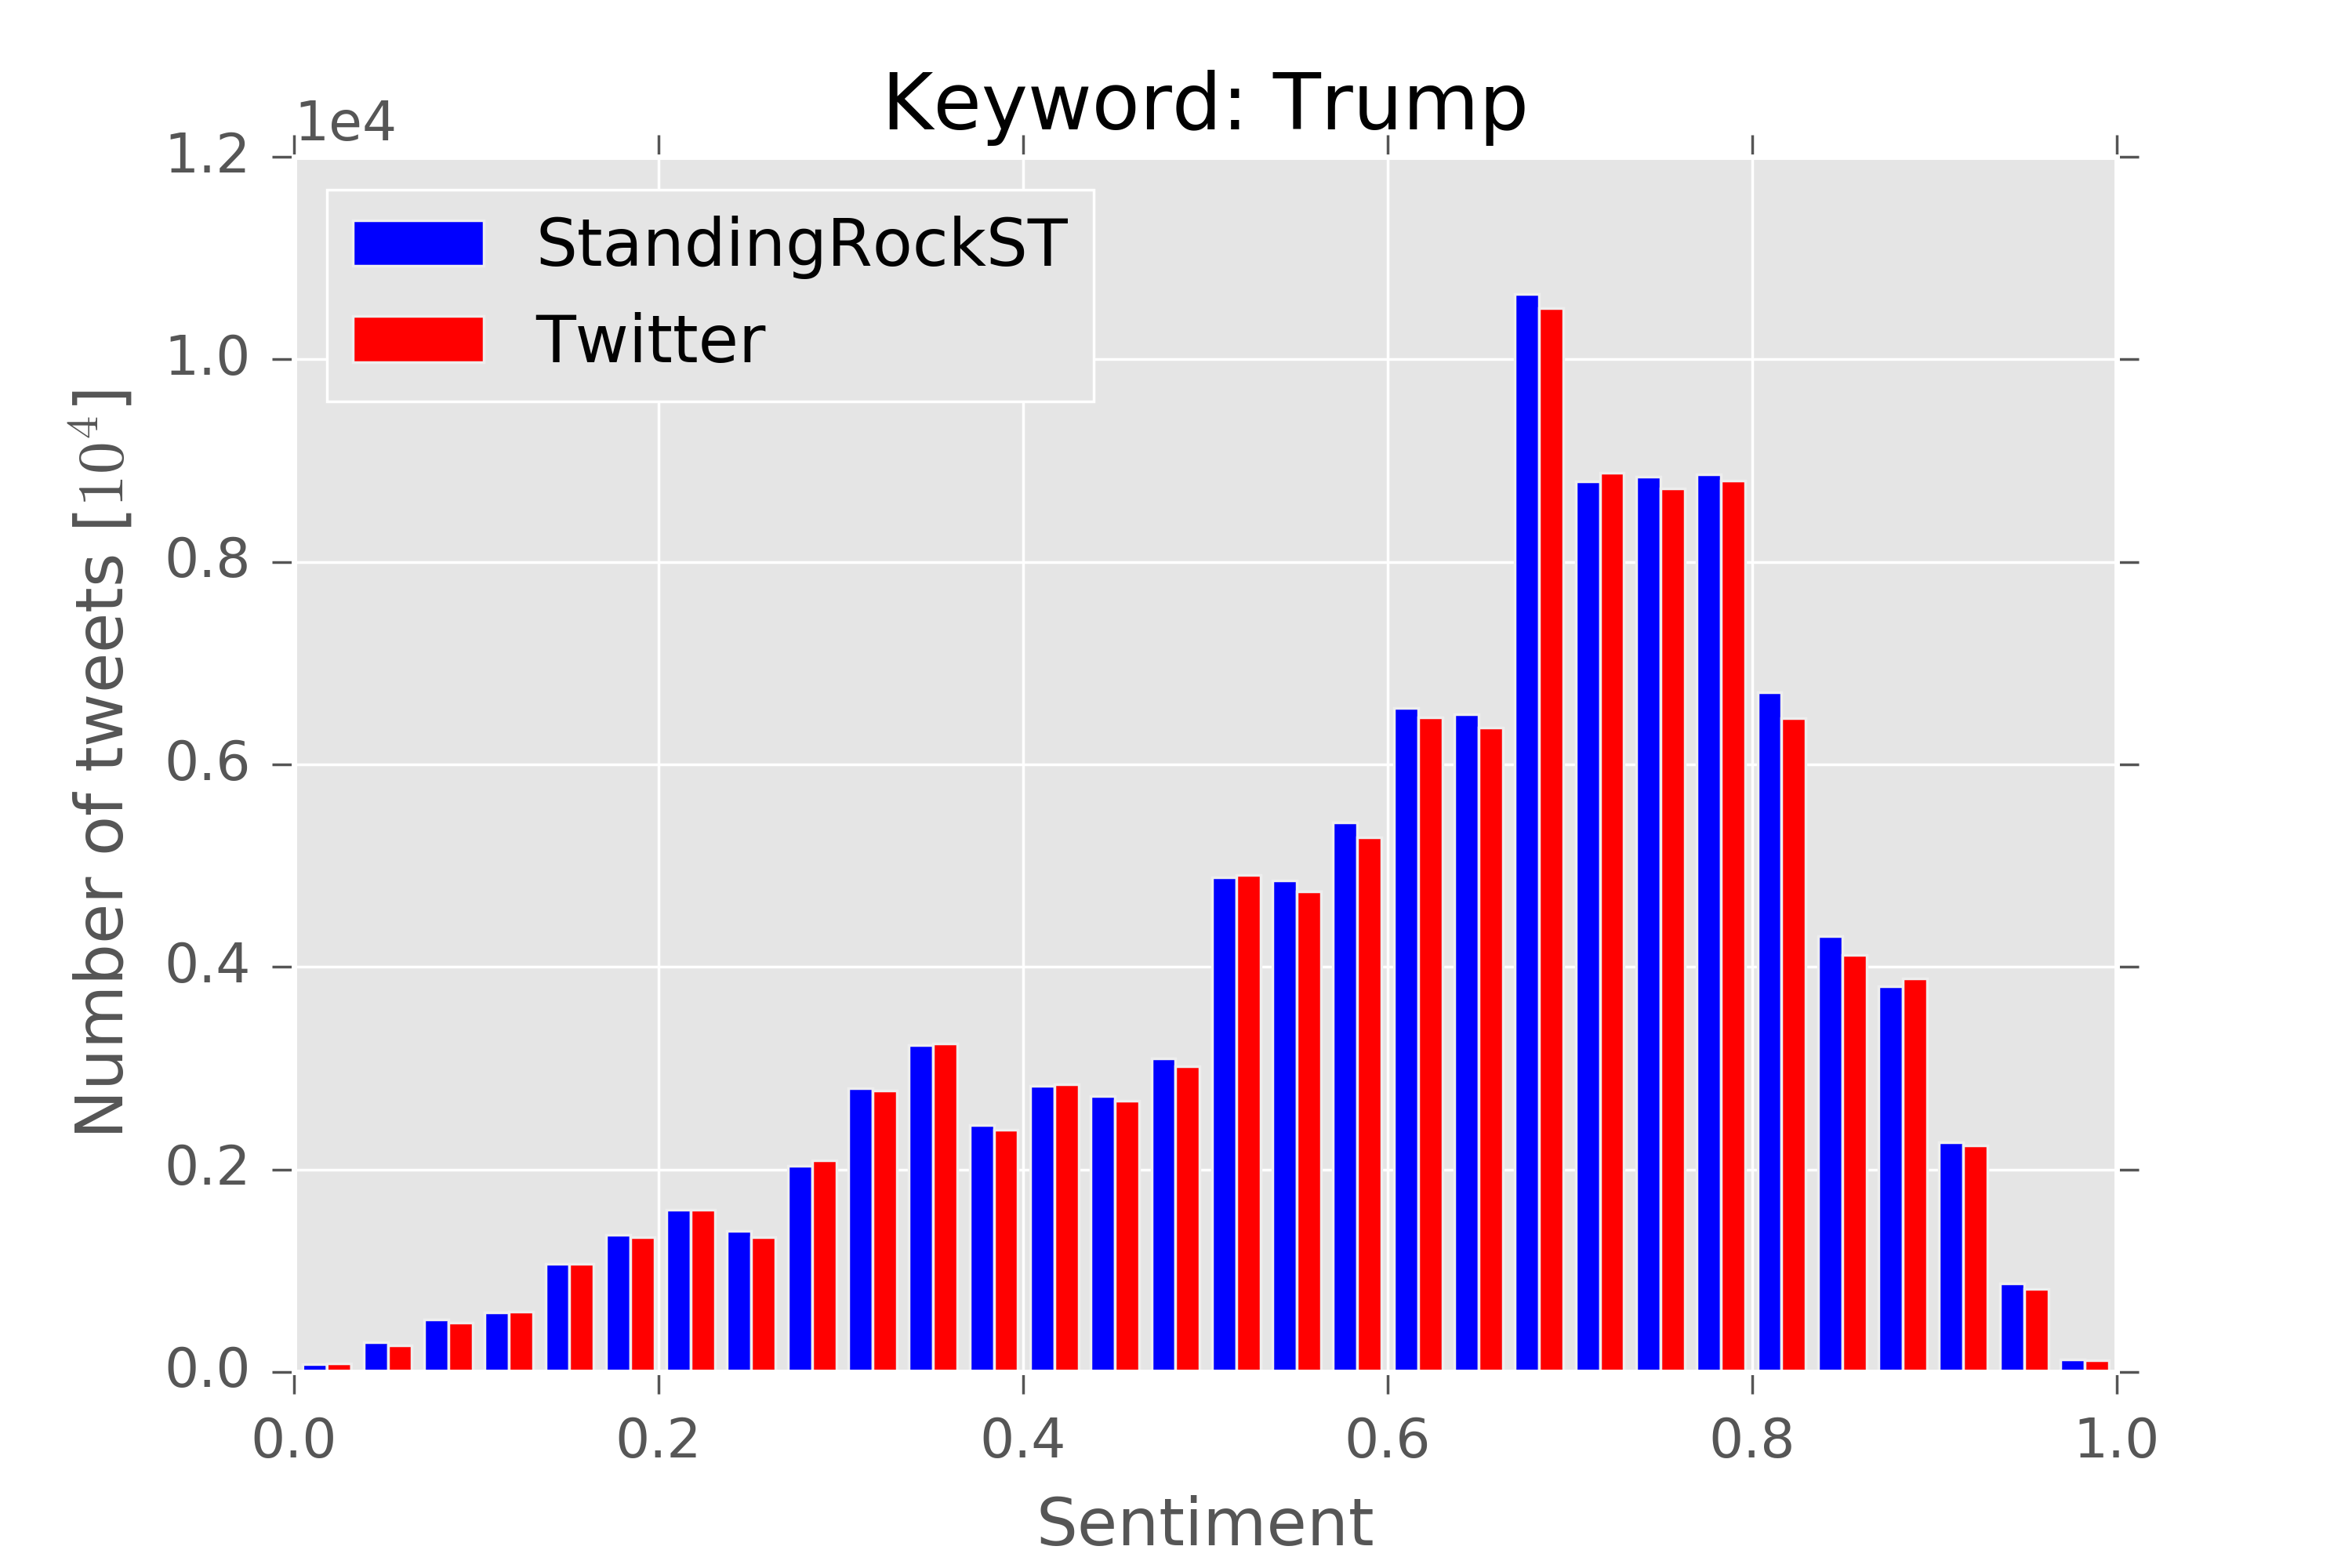
\includegraphics[scale=0.5]{./Pics/indiani-trump.png}
\caption{Histogramy počtu tweetů u skupin s klíčovým slovem \textit{\uv{Trump}}.}
\label{fig:indiani-trump}
\end{figure}

Ať jsme očekávali spíše kladné, nebo záporné příspěvky viditelné uživateli sledující Twitterovou stránku \textit{StandingRockST}, ani k jedné z těchto dvou variant nedošlo. Místo toho je z histogramu \autoref{fig:indiani-trump} patrné, že mají viditelné příspěvky s klíčovým slovem \textit{\uv{Trump}} u \textit{StandingRockST} stejné množství a~sentiment jako pří náhodném výběru z \textit{Twitteru}.

\subsection{Shrnutí pozorování}
\noindent i~přesto, že účelem našich měření bylo spíše ukázat funkce nové metody a~na příkladech prezentovat její klady i~zápory, můžeme si povšimnout několika za\-jí\-ma\-vých poznatků o~samotné \textit{filter bubble}. Výsledky všech měření s klíčovým slovem \textit{\uv{Trump}} v kapitole \fullref{subsec:Trump} pro nás byly velmi překvapující a~v rozporu s naším očekáváním. Počet příspěvků i~rozložení jejich sentimentu byli totožné ve všech měřených skupinách. To i~přes to, že u některých jsme očekávali velkou diversitu a~ohrožení objektivity.

Narozdíl od toho, měření s klíčovým slovem \textit{\uv{abortion}} v kapitole \fullref{subsec:abortion} ukázalo ohrožení informační bublinou u skupiny \textit{Everyday Feminism}. Ta příjmala mnohem větší množství příspěvků s daným klíčovým slovem a~zároveň rozložení sentimentu těchto příspěvků bylo rozdílné od ostatních měřených skupin.

I z takto malého množství pozorování se odvažujeme vyslovit hypotézu. My\-slí\-me si, že \textit{filter bubble} nemůže vzniknout v případě, kdy hovoříme o~obecně velmi diskutovaném tématu. Zato u témat, která nejsou rozšířená dostatečně toto riziko hrozí.

Dle našeho názoru, důvod, proč u velmi rozšířených témat nehrozí \textit{filter bubble} je dostatečně velká konektivita\footnote{Slovem \textit{\uv{dostatečně}} je myšlena takové konektivita, která zaručí dostatečnou ochranu před \textit{filter bubble}.} uživatelů Twitteru. Velmi jedoduše řečeno, my\-slí\-me si, že každý uživatel Twitteru sleduje takové množství lidí, že jsou mezi nimi tací, kteří podporují \textit{Trumpa} i~tací, kteří ho nepodporují. Zato u témat, která jsou méně rozšířená hrozí ohrožení \textit{informační bublinou} právě proto, že nejsou diskutována ve všech skupinách společnosti.

Takovouto domněnku jsme v literatuře zatím nezaznamenali. Je naprosto zřejmé, že vyžaduje ještě další zkoumání a~několika málo měřeními jsme ji dostatečně neobhájili. Jistě se stane předmětem našeho dalšího vyzkumu, jak po praktické stránce měření, tak teoretické stránce, kde bychom rádi zakomponovali myšlenku o~tzv. \textit{assortative mixing}~\cite{AssortativeMixing-soc, AssortativeMixing-E}.

Při užívání nové metody se také ukázalo, že \textit{informační bublinou} je zavislá také na tématu. Ukázali jsme, že existují různé oblasti společenského zájmu, které nemusí být zasaženy \textit{homogenitou} do stejné míry.

\subsection{Diskuze metody}
\noindent V předchozích částech jsme představili novou metodu studia informační bubliny, kterou bychom chtěli zajistit přesnější a~přímější měření tohoto efektu. Samozřejmě má však své nedostatky, které se cítíme být povinni zde sdělit.

Způsob, kterým vybírame členy různých skupin je založen na náhodném vý\-bě\-ru uživatelů sledujicích dominantní stránky sdružující uživatele s podobnými zájmy. Tato metoda může být velmi nespolehlivá hned z několika důvodů. Pře\-váž\-ně je tomu tak proto, že jistě existuje mnoho uživatelů, kteří stránku sledují a~zároveň nejsou jejími přímými podporovateli. Bohužel jsme nepřišli na způsob jak tomuto zabránit. Částečně tomu však předcházíme tím, že veškeré měření je na relativně velkém vzorku uživatelů. Proto stačí předpokládat, že statisticky významnější množství splňuje naše nároky, což není nijak nereálný předpoklad.

Někdo by mohl poukázat na to, že ve skutečnosti neměříme \textit{filter bubble}, ale pouze sentiment příspěvků viditelných danou skupinou. Toto tvrzení je samozřejmě naprosto pravdivé. Je však třeba uvědomit si, že zatím nikdo nepříšel s dostatečně rozumnou mírou \textit{informační bubliny}, není proto možné ji přímo měřit. Předmětem našeho měření je spíše původce \textit{informační bublinou}.

Z kladných vlastností je jistě velmi podstatné to, že při použití naší metody je možné užití velké množství vzorků. To kladně příspívá k rozeznávání šumu v datech od skutečně významných poznatků.

Dále jiště stojí za zmínku, že \textit{filter bubble} měříme přímo v místě jejího výskytu a~ne v uměle vytvořeném prostředí, jako většina z přechozích studií. Je nám také umožněno studium pouze v rámci určitého tématu.

% ##############################################################################
% ##############################################################################
\newpage
\section{Závěr}
\noindent V první části práce jsme přiblížili problematiku informační bubliny, její dopady na společnost v makroskopickém měřítku a~dosud provedené studie.  Odtud jsme se přesunuli na technickou složku práce, kde jsme rozebrali veškeré detaily od stahování dat ze sociální sítě Twitter, přes aplikaci sentimentální analýzy v praxi až po samotnou konstrukci celého měření.

Jak jsme se v úvodu zmínili, cílem naší práce bylo vyvinutí metody, za pomocí které bychom mohli analyzovat míru postižení společnosti informační bublinou. Tohoto cíle jsme dosáhli, podařilo se nám vyvinout zmíněnou metodu. Výsledky měření dopadly, navzdory naším předpokladům, polarizovaně jen v některých případech. V souvislosti s tím jsme vyslovili hypotézu o~vzniku a~ohrožení \textit{informační bublinou}.

Novou metodu volně zpřístupňujeme, abychom umožnili její snadné užití ve výzkumu. Dále budeme provádět více měření a~pokusíme se obhájit, případně vyvrátit naši hypotézu. Výzvou je také nalezení vztahu mezi tzv. \textit{assortative mixing} a~\textit{filter bubble} ve smyslu, ve kterém ji prezentujeme v naší hypotéze.

Při žádné části výzkumu nebylo nijak porušeno právo a~soukromí žádného ze zkoumaných uživatelů.


\newpage
\begin{thebibliography}{99}

    \bibitem{TensorFlow}
    ABADI, Martín, et al. \textit{TensorFlow: Large-Scale Machine Learning on Heterogeneous Distributed Systems}. (2015). arXiv:1603.04467. Dostupné také z: \url{https://arxiv.org/abs/1603.04467}

    \bibitem{whyNotFb}
    BARTHEL, Michael, Elisa SHEARER, Jeffrey GOTTFRIED a~Amy MITCHELL. \textit{The Evolving Role of News on Twitter and Facebook} [online]. Pew Research Center, 2015 [cit. 2017-01-22]. Dostupné z: \url{http://www.journalism.org/2015/07/14/the-evolving-role-of-news-on-twitter-and-facebook/}

    \bibitem{NLTKbook}
    BIRD, Steven, Ewan KLEIN a~Edward LOPER. \textit{Natural language processing with Python}. Beijing: O'Reilly, 2009. ISBN 978-0-596-51649-9. Dostupné také z: \url{http://www.nltk.org/book/}

    \bibitem{BreakingTheFilterBubble}
    BOZDAG, Engin a~Jeroen VAN DEN HOVEN. Breaking the filter bubble: democracy and design. \textit{Ethics and Information Technology}. 2015, \textbf{17}(4), 249-265. DOI: 10.1007/s10676-015-9380-y. ISSN 1388-1957. Dostupné také z: \url{http://link.springer.com/10.1007/s10676-015-9380-y}

    \bibitem{keras}
    CHOLLET, Fran\c{c}ois. \textit{Keras}. GitHub 2015 [online]. [cit. 2017-01-22]. Dostupné také z: \url{https://github.com/fchollet/keras}

    \bibitem{YouTube}
    DAVIDSON, James, et al. The YouTube video recommendation system. \textit{Proceedings of the fourth ACM conference on Recommender systems - RecSys '10}. New York, New York, USA: ACM Press, 2010. DOI: 10.1145/1864708.1864770. ISBN 9781605589060. Dostupné také z: \url{http://portal.acm.org/citation.cfm?doid=1864708.1864770}

    \bibitem{myRepo}
    DOSTÁL, Jakub. \textit{FilterBubble-Twitter}. GitHub 2017 [online]. Dostupné také z: \url{https://github.com/DostalJ/FilterBubble-Twitter}

    \bibitem{WordEmbedding2}
    GOLDBERG, Yoav a~Omer LEVY. Word2vec Explained: deriving Mikolov et al.'s negative-sampling word-embedding method. \textit{ArXiv: Computation and Language}. 2014. arxiv:1402.3722. Dostupné také z: \url{https://arxiv.org/abs/1402.3722}

    \bibitem{TheImpactOfFilterBubble}
    GOTTRON, Thomas a~Felix SCHWAGEREIT. The Impact of the Filter Bubble -- a~Simulation Based Framework for Measuring Personalisation Macro Effects in Online Communities. \textit{ARXIV: Computer Science - Social and Information Networks}. 2016, \textbf{2016}. arXiv161206551G. Dostupné také z: \url{https://arxiv.org/abs/1612.06551\#}

    \bibitem{tweepy}
    HILL, Aaron a~Joshua ROESSLEIN. \textit{Tweepy}. Github 2015 [online]. [cit. 2017-01-22]. Dostupné z: \url{https://github.com/tweepy/tweepy}

    \bibitem{Huberman2012-2-15} % big data anywhere
    HUBERMAN, Bernardo A. Sociology of science: Big data deserve a~bigger audience. \textit{Nature}. 2012-2-15, \textbf{482}(7385), 308-308. DOI: 10.1038/482308d. ISSN 0028-0836. Dostupné také z: \url{http://www.nature.com/doifinder/10.1038/482308d}

    \bibitem{BeyondFilterBubble}
    LIAO, Q. Vera a~Wai-Tat FU. Beyond the filter bubble: Interactive effects of perceived threat and topic involvement on selective exposure to information. \textit{Proceedings of the SIGCHI Conference on Human Factors in Computing Systems - CHI '13}. New York, New York, USA: ACM Press, 2013, 2359-2368. DOI: 10.1145/2470654.2481326. ISBN 9781450318990. Dostupné také z: \url{http://dl.acm.org/citation.cfm?doid=2470654.2481326}

    \bibitem{Amazon}
    LINDEN, G., B. SMITH a~J. YORK. Amazon.com recommendations: item-to-item collaborative filtering. \textit{IEEE Internet Computing}. 2003, \textbf{7}(1), 76-80. DOI: 10.1109/MIC.2003.1167344. ISSN 1089-7801. Dostupné také z: \url{http://ieeexplore.ieee.org/document/1167344/}

    \bibitem{TwitterRecomendation}
    KIM, Younghoon a~Kyuseok SHIM. TWITOBI: a~Recommendation System for Twitter Using Probabilistic Modeling. \textit{2011 IEEE 11th International Conference on Data Mining}. IEEE, 2011, , 340-349. DOI: 10.1109/ICDM.2011.150. ISBN 978-1-4577-2075-8. Dostupné také z: \url{http://ieeexplore.ieee.org/document/6137238/}

    \bibitem{Mathioudakis2010}
    MATHIOUDAKIS, Michael a~Nick KOUDAS. TwitterMonitor. \textit{Proceedings of the 2010 international conference on Management of data - SIGMOD '10}. New York, New York, USA: ACM Press, 2010, \textbf{2010}, 1155-1158. DOI: 10.1145/1807167.1807306. ISBN 9781450300322. Dostupné také z: \url{http://portal.acm.org/citation.cfm?doid=1807167.1807306}

    \bibitem{McFarland2016} % big data in sociology
    MCFARLAND, Daniel A., Kevin LEWIS a~Amir GOLDBERG. Sociology in the Era of Big Data: The Ascent of Forensic Social Science. \textit{The American Sociologist}. 2016, \textbf{47}(1), 12-35. DOI: 10.1007/s12108-015-9291-8. ISSN 0003-1232. Dostupné také z: \url{http://link.springer.com/10.1007/s12108-015-9291-8}

    \bibitem{AssortativeMixing-soc}
    MCPHERSON, Miller, Lynn SMITH-LOVIN a~James M COOK. Birds of a~Feather: Homophily in Social Networks. \textit{Annual Review of Sociology}. 2001, \textbf{27}(1), 415-444. DOI: 10.1146/annurev.soc.27.1.415. ISSN 0360-0572. Dostupné také z: \url{http://www.annualreviews.org/doi/10.1146/annurev.soc.27.1.415}

    \bibitem{WordEmbedding1}
    MIKOLOV, Tomas, Ilya SUTSKEVER, Kai CHEN, Greg CORRADO a~Dean JEFF. Distributed Representations of Words and Phrases and their Compositionality. \textit{Advances in Neural Information Processing Systems}. Curran Associates, 2013, (26), 3111-3119. Dostupné také z: \url{https://arxiv.org/abs/1310.4546}

    \bibitem{AssortativeMixing-E}
    NEWMAN, M. E. J. Mixing patterns in networks. \textit{Physical Review E}. 2003, \textbf{67}(2). DOI: 10.1103/PhysRevE.67.026126. ISSN 1063-651x. Dostupné také z: \url{https://arxiv.org/abs/cond-mat/0209450}

    \bibitem{HumanVsMachineLearning}
    PANG, Bo, Lillian LEE a~Shivakumar VAITHYANATHAN. Thumbs up?: sentiment classification using machine learning techniques. \textit{Proceedings of the ACL-02 conference on Empirical methods in natural language processing - EMNLP '02}. Morristown, NJ, USA: Association for Computational Linguistics, 2002, \textbf{2002}(10), 79-86. DOI: 10.3115/1118693.1118704. Dostupné také z: \url{http://portal.acm.org/citation.cfm?doid=1118693.1118704}

    \bibitem{DemocracyOnline}
    PAPACHARISSI, Zizi. Democracy online: civility, politeness, and the democratic potential of online political discussion groups. \textit{New Media}. 2004, \textbf{6}(2), 259-283. DOI: 10.1177/1461444804041444. ISSN 1461-4448. Dostupné také z: \url{http://journals.sagepub.com/doi/10.1177/1461444804041444}

    \bibitem{PariserTed}
    PARISER, Eli. (2011). \textit{Beware online "filter bubbles"} [online]. Dostupné z \url{https://www.ted.com/talks/eli_pariser_beware_online_filter_bubbles}

    \bibitem{Pariser2011}
    PARISER, Eli. \textit{The filter bubble: what the Internet is hiding from you}. New York: Penguin Press, 2011. ISBN 15-942-0300-8.

    \bibitem{whyNewsOnTwitter}
    ROSENSTIEL, T., et al. Twitter and the News: How people use the social network to learn about the world. \textit{American Press Institute: Insights, tools and research to advance journalism} [online]. 2015, \textbf{2015} [cit. 2017-01-22]. Dostupné z: \url{https://www.americanpressinstitute.org/publications/reports/survey-research/how-people-use-twitter-news/}

    \bibitem{TwitterData1}
    SANDERS, Niek. \textit{Twitter Sentiment Corpus}. Sanders Analytics, 2011. Dostupné také z: \url{http://www.sananalytics.com/lab/twitter-sentiment/}

    \bibitem{TwitterSentAnalysis}
    SEVERYN, Aliaksei a~Alessandro MOSCHITTI. Twitter Sentiment Analysis with Deep Convolutional Neural Networks. \textit{Proceedings of the 38th International ACM SIGIR Conference on Research and Development in Information Retrieval - SIGIR '15}. New York, New York, USA: ACM Press, 2015, \textbf{2015}, 959-962. DOI: 10.1145/2766462.2767830. ISBN 9781450336215. Dostupné také z: \url{http://dl.acm.org/citation.cfm?doid=2766462.2767830}

    \bibitem{Shah2015-04-09} % big data in sociology
    SHAH, D. V., J. N. CAPPELLA a~W. R. NEUMAN. Big Data, Digital Media, and Computational Social Science: Possibilities and Perils. \textit{The ANNALS of the American Academy of Political and Social Science}. 2015, \textbf{659}(1), 6-13. DOI: 10.1177/0002716215572084. ISSN 0002-7162. Dostupné také z: \url{http://ann.sagepub.com/cgi/doi/10.1177/0002716215572084}

    \bibitem{Tinati2014} % big data in sociology
    TINATI, Ramine, Susan HALFORD, Leslie CARR a~Catherine POPE. Big Data: Methodological Challenges and Approaches for Sociological Analysis. \textit{Sociology}. 2014, \textbf{48}(4), 663-681. DOI: 10.1177/0038038513511561. ISSN 0038-0385. Dostupné také z: \url{http://journals.sagepub.com/doi/10.1177/0038038513511561}

    \bibitem{twitterAPI}
    Twitter, API Overview. \textit{Twitter Developer Documentation} [online]. Twitter, 2016 [cit. 2017-01-22]. Dostupné z: \url{https://dev.twitter.com/overview/api}

    \bibitem{TwitterData2}
    University of Michigan, \textit{UMICH SI650: Sentiment Classification}. University of Michigan SI650, 2011. Dostupné také z: \url{https://inclass.kaggle.com/c/si650winter11/data}

    \bibitem{CNN}
    YOON, Kim. Convolutional Neural Networks for Sentence Classification. \textit{ArXiv: Computation and Language}. arXiv, 2014. arXiv:1408.5882v2. Dostupné také z: \url{https://arxiv.org/abs/1408.5882}

\end{thebibliography}
\end{document}
